%=======================================================================
% Latex template for SPAA 2012
%=======================================================================

% remember to compile with dvips -t letter for US letter style

%\documentclass[preprint,nocopyrightspace]{sigplanconf}
\documentclass[pldi, 10pt, nocopyrightspace]{sigplanconf}
%\documentclass{llncs} 
%\documentclass[10pt]{IEEEtran}
%\documentclass[times,10pt,twocolumn]{article} 

% American letter size:
%\textwidth6.5in \textheight9in \oddsidemargin 0pt \evensidemargin 0pt
%\topmargin -47pt

%\usepackage[sort&compress]{natbib}
\usepackage{bussproofs}
\usepackage{ulem}
%\usepackage[margin=0.5in]{geometry}
\usepackage{colonequals}
\usepackage{mathtools}
\usepackage{times}
\usepackage{color}
\usepackage{comment}
\usepackage{amsmath}
\usepackage{amssymb}
\usepackage{amsthm}
\usepackage{float}
\usepackage{multirow}
\usepackage{alltt}
\usepackage{semantic}
\usepackage{caption}
\usepackage{subcaption}
\DeclareCaptionType{copyrightbox}
\captionsetup{compatibility=false}
\usepackage{boxedminipage}
\usepackage{listings}
\usepackage{lstlangcoq}
\usepackage{multirow}
%\usepackage{cite}
\usepackage{url}
\usepackage{amsfonts}

\usepackage[pdftex]{graphicx}
\graphicspath{{figures/}}
\DeclareGraphicsExtensions{.pdf,.jpg,.png}

%{\obeyspaces\gdef {\ }}

\begin{document}
%\special{papersize=8.5in,11in}
\setlength{\pdfpageheight}{\paperheight}
\setlength{\pdfpagewidth}{\paperwidth}

% Uncomment one of the following two, if you are not going for the 
% traditional copyright transfer agreement.

%\exclusivelicense                % ACM gets exclusive license to publish, 
                                  % you retain copyright

%\permissiontopublish             % ACM gets nonexclusive license to publish
                                  % (paid open-access papers, 
                                  % short abstracts)

%\titlebanner{Draft}
\preprintfooter{Modular Deductive Verification of Multiprocessor Hardware Designs}


\newcommand{\ndave}[1]{\color{blue}{#1: ---- \textbf{Nirav}}}
\newcommand{\murali}[1]{\xxx{#1: ---- \textbf{Murali}}}
\newcommand{\adam}[1]{\xxx{#1: ---- \textbf{Adam}}}

%\spnewtheorem{thm}{Theorem}{\bfseries}{\normalfont}
%\spnewtheorem{defn}{Definition}{\bfseries}{\normalfont}
%\spnewtheorem{inv}{Invariant}{\bfseries}{\normalfont}
\newtheorem{theorem}{Theorem}
\newtheorem{corollary}{Corollary}
\newtheorem{defn}{Definition}
\newtheorem{lemma}{Lemma}
\newtheorem{inv}{Invariant}

\newcommand{\qs}{\mathit{qs}}
\newcommand{\rs}{\mathit{rs}}
\newcommand{\noSpec}{\mathsf{noSpec}}
\newcommand{\f}{\text{noSpec}}
\newcommand{\g}{\text{store}}
\newcommand{\Id}{\mathit{Id}}
\newcommand{\trans}[3]{(#2) \xrightarrow[\text{#1}]{} (#3) }
\newcommand{\transn}[3]{(#2) \xrightarrow[\text{#1}]{}\\ (#3) }
\newcommand{\transs}[3]{(#2) \xrightarrow[\text{#1}]{}^{*} (#3) }
\newcommand{\transsn}[3]{(#2) \xrightarrow[\text{#1}]{}^{*}\\ (#3) }

\newcommand{\smulti}[2]{#2^{#1}}
\newcommand{\multi}[2]{(\{1\ldots #1\}\rightarrow #2)}
\newcommand{\multit}[2]{\xrightarrow[\multi{#1}{#2}]{}}

\newcommand{\toM}{\mathsf{ToM}}
\newcommand{\toP}{\mathsf{ToP}}
\newcommand{\iom}[5]{(#2) \xrightarrow[\text{#1}]{(#4, #5)} (#3) }
\newcommand{\ioe}[3]{(#2) \xrightarrow[\text{#1}]{} (#3) }
\newcommand{\ioxe}[3]{\left(\begin{array}{l}#2\end{array}\right) 
\xrightarrow[\text{#1}]{} \left(\begin{array}{l}#3\end{array}\right) }
\newcommand{\ioen}[3]{(#2) \xrightarrow[\text{#1}]{\epsilon}\\ (#3) }
\newcommand{\ioens}[3]{(#2) {\xrightarrow[\text{#1}]{\epsilon}}^{*} (#3) }
\newcommand{\ioensn}[3]{(#2) {\xrightarrow[\text{#1}]{\epsilon}}^{*}\\ (#3) }
\newcommand{\ior}[4]{(#2) \xrightarrow[\text{#1}]{\text{ToM} (#4)} (#3) }
\newcommand{\iol}[4]{(#2) \xrightarrow[\text{#1}]{\text{ToP} (#4)} (#3) }
\newcommand{\iorn}[5]{(#2) \xrightarrow[\text{#1}]{#4, \text{ToM} (#5)} (#3) }
\newcommand{\ioln}[5]{(#2) \xrightarrow[\text{#1}]{#4, \text{ToP} (#5)} (#3) }
\newcommand{\io}[4]{(#2) \xrightarrow[\text{#1}]{#4} (#3) }
\newcommand{\ios}[4]{(#2) {\xrightarrow[\text{#1}]{#4}}^{*} (#3) }

%\newcommand{\iom}[5]{(#2, (#4)) \xrightarrow[\text{#1}]{} (#3, (#5)) }
%\newcommand{\ioe}[3]{(#2, \epsilon) \xrightarrow[\text{#1}]{} (#3, \epsilon) }
%\newcommand{\ioen}[3]{(#2, \epsilon) \xrightarrow[\text{#1}]{}\\ (#3, \epsilon) }
%\newcommand{\ioens}[3]{(#2, \epsilon) \xrightarrow[\text{#1}]{}^{*} (#3, \epsilon) }
%\newcommand{\ioensn}[3]{(#2, \epsilon) \xrightarrow[\text{#1}]{}^{*}\\ (#3, \epsilon) }
%\newcommand{\ior}[4]{(#2, \epsilon) \xrightarrow[\text{#1}]{} (#3, (#4)) }
%\newcommand{\iol}[4]{(#2, (#4)) \xrightarrow[\text{#1}]{} (#3, \epsilon) }
%\newcommand{\io}[4]{(#2, h) \xrightarrow[\text{#1}]{} (#3, (#4) \coloncolon h) }

\newcommand{\dt}{\mathit{d}}
\newcommand{\ch}{\mathit{ch}}
\newcommand{\s}{\mathit{cs}}
\newcommand{\dst}{\mathit{dir}}
\newcommand{\wt}{\mathit{w}}
\newcommand{\wts}{\mathit{wts}}
\newcommand{\dwt}{\mathit{dirw}}
\newcommand{\dwts}{\mathit{dwts}}
\newcommand{\compat}{\mathsf{dirCompat}}

\newcommand{\Real}{\mathit{NonSpec}}
\newcommand{\Spec}{\mathit{Spec}}
\newcommand{\Set}[1]{\text{Set}(#1)}
\newcommand{\id}{\mathit{id}}
\newcommand{\inp}{\mathit{ins}}
\newcommand{\outp}{\mathit{outs}}
\newcommand{\un}{\mathit{Simp}}
\newcommand{\stream}[1]{\mathit{Stream}(#1)}
\newcommand{\mem}{\text{Mem}}
\newcommand{\cache}{\text{Cache}}
\newcommand{\pc}{\mathit{pc}}
\newcommand{\mult}{\text{Mult}}
\newcommand{\simps}{\mathit{Simps}}
\newcommand{\specs}{\mathit{Specs}}
\newcommand{\dcs}{\mathit{Decs}}
\newcommand{\dce}{\mathit{Dec}}
\newcommand{\spe}{\mathit{Spec}}
\newcommand{\wait}{\mathit{wait}}
\newcommand{\sta}{\mathit{state}}
\newcommand{\ptm}{\mathit{p2m}}
\newcommand{\mtp}{\mathit{m2p}}
\newcommand{\rob}{\mathit{rob}}
\newcommand{\ppc}{\mathit{bp}}
\newcommand{\curPpc}{\mathsf{curPpc}}
\newcommand{\nextPpc}{\mathsf{nextPpc}}
\newcommand{\add}{\mathsf{insert}}
\newcommand{\compute}{\mathsf{compute}}
\newcommand{\retire}{\mathsf{retire}}
\newcommand{\commit}{\mathsf{commit}}
\newcommand{\comm}{\text{Com}}

\newcommand{\dec}{\mathsf{dec}}
\newcommand{\exec}{\mathsf{exec}}
\newcommand{\st}{\mathsf{St}}
\newcommand{\nm}{\mathsf{Nm}}
\newcommand{\req}{\mathsf{Rq}}
\newcommand{\rep}{\mathsf{Rp}}
\newcommand{\Tag}{\mathsf{Tag}}

\newcommand{\proc}{\mathsf{Proc}}
\newcommand{\prog}{\mathsf{prog}}
\newcommand{\ld}{\mathsf{Ld}}
\newcommand{\upd}{\mathsf{upd}}
\newcommand{\updM}{\mathsf{updM}}
\newcommand{\abort}{\mathsf{Abort}}
\newcommand{\get}{\mathsf{get}}
\newcommand{\setBp}{\mathsf{setNextPpc}}
\newcommand{\set}{\mathsf{set}}
\newcommand{\spc}{\mathsf{Spec}}
\newcommand{\Next}{\mathsf{next}}

\newcommand{\toProc}{\mathsf{toProc}}
\newcommand{\fromProc}{\mathsf{fromProc}}
%\spnewtheorem*{adefn}{Definition}
%\spnewtheorem{thm}{Theorem}
%\spnewtheorem*{athm}{Definition}
\newcommand{\teq}{\mathsftt{=}}
\newcommand{\eg}{\textit{e.g.,}}
\newcommand{\etc}{\textit{etc.}}
\newcommand{\ie}{\textit{i.e.,}}
\newcommand{\etal}{\textit{et al.}}
\newcommand{\viz}{\textit{viz},} 
\newcommand{\xxx}[1]{{\textbf{\color{blue}{#1}}}}
%
\newcommand{\Ld}{\mathsftt{Load}}
\newcommand{\St}{\mathsftt{Store}}
\newcommand{\fulllabel}[1]{\label{#1}\textit{#1}}
\newcommand{\Ow}{\textit{O}}
\newcommand{\sibling}{\textit{sibling}}
\newcommand{\clean}{\textit{clean}}
\newcommand{\emp}{\(\epsilon\)}
\newcommand{\getReq}{\textit{getReq}}
\newcommand{\match}{\mathsftt{match }}
\newcommand{\with}{\mathsftt{ with}}
\newcommand{\myend}{\mathsftt{end}}
\newcommand{\mylet}{\mathsftt{let }}
\newcommand{\myin}{\mathsftt{ in }}
\newcommand{\myif}{\mathsftt{if }}
\newcommand{\mythen}{\mathsftt{ then }}
\newcommand{\myelse}{\mathsftt{ else }}
\newcommand{\leaf}{\textit{leaf}}
\newcommand{\pos}{\textit{seqNum}}
\newcommand{\resp}{\rep}
\newcommand{\addr}{\textit{addr}}
\newcommand{\tme}{\textit{time}}
\newcommand{\initData}{\textit{initData}}
\newcommand{\fst}{\mathsftt{fst}}
\newcommand{\snd}{\mathsftt{snd}}
\newcommand{\Request}{\textit{ProcReq}}
\newcommand{\Response}{\textit{ProcResp}}
\newcommand{\reqFn}{\textit{reqFn}}
\newcommand{\respFn}{\textit{respFn}}
\newcommand{\addrQ}{\textit{addrP}}
\newcommand{\desc}{\textit{desc}}
\newcommand{\typ}{\textit{type}}
\newcommand{\dataQ}{\textit{dataP}}
\newcommand{\labelR}{\textit{labelR}}
\newcommand{\procR}{\textit{procR}}
\newcommand{\idxR}{\textit{indexR}}
\newcommand{\dataR}{\textit{dataR}}
\newcommand{\timeR}{\textit{timeR}}
\newcommand{\from}{\textit{from}}
\newcommand{\myto}{\textit{to}}
\newcommand{\data}{\textit{data}}
\newcommand{\Req}{\textit{Req}}
\newcommand{\Resp}{\textit{Resp}}
\newcommand{\Mo}{\textit{M}}
\newcommand{\Sh}{\textit{S}}
\newcommand{\In}{\textit{I}}
\newcommand{\cpReq}{\textit{c2pReq}}
\newcommand{\cpResp}{\textit{c2pResp}}
\newcommand{\ptc}{\textit{p2c}}
\newcommand{\False}{\mathit{False}}
\newcommand{\True}{\mathit{True}}
\newcommand{\Reqcp}{\textit{Req-c2p}}
\newcommand{\Respcp}{\textit{Resp-c2p}}
\newcommand{\Mpc}{\textit{Mesg-p2c}}
\newcommand{\state}{\textit{state}}
\newcommand{\parent}{\textit{parent}}
\newcommand{\dstate}{\textit{dstate}}
\newcommand{\waitS}{\textit{waitS}}
\newcommand{\dwait}{\textit{dwait}}
\newcommand{\dwaitS}{\textit{dwaitS}}
\newcommand{\enq}{\mathsf{enq}}
\newcommand{\deq}{\mathsf{deq}}
\newcommand{\pop}{\mathsf{pop}}
\newcommand{\avail}{\textit{avail}}
\newcommand{\first}{\mathsf{first}}
\newcommand{\ite}[3]{\mathsf{if}(#1) \; \mathsf{then} \; #2 \; \mathsf{else} \; #3}

%\mathlig{@->}{\rightarrow}
%\mathlig{@<}{\langle}
%\mathlig{@>}{\rangle}
%\mathlig{@|->}{\mapsto}

%\begin{titlepage}

\title{Modular Deductive Verification of Multiprocessor Hardware Designs}

%       {\Large (Regular Submission)}}

%% \authorinfo{}%{Muralidaran Vijayaraghavan}
%%            {}%{Massachusetts Institute of Technology, Cambridge MA, USA}
%%            {}%{vmurali@csail.mit.edu}

%% \authorinfo{}%{Adam Chlipala}
%%            {}%{Massachusetts Institute of Technology, Cambridge MA, USA}
%%            {}%{adamc@csail.mit.edu}

%% \authorinfo{}%{Arvind}
%%            {}%{Massachusetts Institute of Technology, Cambridge MA, USA}
%%            {}%{arvind@csail.mit.edu}

%% \authorinfo{}%{Nirav Dave}
%%            {}%{SRI International}
%%            {}%{ndave@csl.sri.com}

\authorinfo{}{}

\maketitle % \thispagestyle{empty}

%=========================================================================
%  Abstract
%=========================================================================

\begin{abstract}
We present a new framework for modular verification of hardware designs in the
style of the Bluespec language.  That is, we formalize the idea of components
in a hardware design, with well-defined input and output channels; and we show
how to specify and verify components individually, with machine-checked proofs
in the Coq proof assistant.  As a demonstration, we verify a fairly realistic
implementation of a multicore shared-memory system with two types of
components:  memory-system and processor.  Both components include nontrivial
optimizations, with the memory system employing an arbitrary hierarchy of cache
nodes that communicate with each other concurrently, and with the processor
doing speculative execution of many concurrent read operations.  Nonetheless,
we prove that the combined system implements sequential consistency.  One
interesting aspect of the proof is that the memory component is well-specified
to be reusable for systems implementing a variety of weak memory models.  To
our knowledge, our memory-system system proof is the first machine verification
of a cache-coherence protocol parameterized over an arbitrary cache hierarchy,
and our full-system proof is the first machine verification of sequential
consistency for a multicore hardware design that includes caches and
speculative processors.


\end{abstract}

%\bigskip

%\keywords
%memory-models, cache-coherence, processor-reordering


%\end{titlepage}

\section{Introduction}
\label{sec:Introduction}

A modern high-performance, cache-coherent, distributed-memory hardware system is
inherently complex. Such a system implements memory models like sequential
consistency (SC)~\cite{lamport1979make}, Total Store Order (TSO), and
Relaxed Memory Order (RMO)~\cite{weaver1994sparc}, each
of which characterizes how loads and stores may be issued by a processor and
how the shared-memory component responds to these requests.  These systems by
their nature are highly concurrent and nondeterministic.

The goal of this work is to provide a framework for full verification of such
complex hardware systems. Hardware designers already recognize the challenge of
implementing these systems, to such an extent that they have already become some
of the most serious real-world adopters of formal methods.  Hardware
verification is dominated by model-checking, where abstraction techniques are
used to reduce designs to finite state spaces, which can be explored
exhaustively.  There are limits to the construction of sound abstractions, so
verifications of, e.g., cache-coherence protocols have almost always treated
systems with concrete topologies, involving particular finite numbers of caches
and processors. For instance, explicit-state model checking tools like
Murphi~\cite{murphi} or TLC~\cite{tlc} are only able to handle small and
simplified systems, \eg{} a single-level cache hierarchy with three CPUs, two
addresses, and one bit of data. Symbolic model checking techniques have fared
slightly better: McMillan \etal{} have verified a 2-level MSI protocol based on
the Gigamax distributed multiprocessor using SMV~\cite{gigamax}. Optimizations
on these techniques (\eg{} partial order reduction~\cite{part}, symmetry
reduction~\cite{sym1, sym2}, compositional reasoning~\cite{comp, Mccomp, mcc}, \etc{}) scale
the approach further, but they are still unable to handle realistic
hierarchical protocols. We might hope to achieve higher assurance and
understanding of design ideas by verifying \emph{infinite families} of hardware
designs, which resist reduction to finite-state models.  A potential related
benefit is reducing the computational resources required to formally verify a
new design in the family, applying a more general theorem without much new
analysis.

Modularity has long been understood as a key property for effective design and
verification of such complex systems. For the designer, it allows a separation
of concerns, increasing robustness by allowing the behavior encapsulated by a
modular boundary to be realized by multiple implementations, any of which may be
dropped into the system safely. It also allows a greater
parallelization of human design effort, improving development time. Similarly, verification is
simplified, as modular interface agreements provide a natural lemma structure.
This leads us towards a decomposition of the whole system verification
task into lemmas of subsystems, which can be composed in a black-box manner to
produce full-system theorems.

%\xxx{\textbf{Murali's version in red} This works introduces an interface enabling true modular implementation and
%verification of shared memory systems. We want our modular system to permit
%\emph{black-box refinement}, that is, nothing beyond the interface contract can
%be assumed about other modules.  That is, we should be able to describe a
%modular decomposition where we may replace either the processor nodes, the
%memory with locally verified alternatives without changing the correctness of
%our whole system.  To this end, we identify a key property called \emph{store
%atomicity} shared by the memory component of every memory model. This property
%effectively restricts the behavior of the memory sub-system to that of an
%\emph{atomic instantaneous memory}. We prove that this property is in fact what
%is guaranteed using the cache coherence protocols in a multi-processor system
%containing a hierarchy of caches, enabling replacement of the cache hierarchy
%with an atomic instantaneous memory. Similarly, on the processor side, we
%define what is meant to be a correct single processor. These invariants about
%the processor and the memory sub-system remains constant across memory models.
%We show a concrete instance of this framework by proving that a highly
%speculative multi-processor system connected to a coherent cache hierarchy
%implements the sequential consistency memory model.}


In this paper, we introduce \textbf{a new approach to modular,
  deductive verification of hardware designs} at the highest level of
rigor, backed by proofs using the Coq proof assistant.  As a
challenging case study, we focus on \textbf{verifying that a
  particular infinite family of multicore, shared-memory systems
  implements sequential consistency}.  The proof is parametrized over
an unknown number of processors connected to an arbitrary memory
hierarchy with an unknown number of caches in an unknown number of
layers (e.g., L1, L2).  In our design, processors and memory systems
both independently employ intricate optimizations that exploit
opportunities for parallelism.  We are able to prove that each of
those two main components still implements strong enough semantics to
support SC, and then we compose those theorems into a result for the
full system.  Either component may be optimized further without
requiring any changes to the implementation, specification, or proof
of the other.

To structure our hardware verification framework, we import
\emph{labeled transition systems (LTSes)}, a well-studied approach from the
world of concurrent software modeling.  As our unified notion of
specification and proof, we adopt \emph{trace refinement}, which
captures when one concurrent system can only produce observable IO
behaviors that another system could also produce.  Each of our
realistic hardware components is associated with a simpler ``reference
implementation'' that serves as a specification, and we prove that
each realistic component refines its spec.  Thereafter, it is sound to
use the simpler spec component in reasoning about the behavior of the
system.

Each key component of our case-study system has a simple spec: the
ideal memory responds instantly and atomically to each load or store
request, and the ideal processor executes instructions in order with
no speculation.  The optimized implementation of each is much more
complicated: the cache-hierarchy memory system potentially allows
every cache to be busy simultaneously computing and sending messages,
and the optimized speculative processor sends multiple load requests
to the memory at once, without waiting for responses first.  The meat
of the verification is in showing that each optimized component
refines its simpler counterpart.  After each such proof, we may in
effect substitute the optimized version for the simple version in a
black-box way within a design, with a full guarantee of soundness.

LTSes as hardware descriptions are an established
idea~\cite{HoeArvind:TRSSynthesis1, Hoe:TCAD}, and there are
compilers that convert LTSes into efficient hardware.  Our work is
based on the Bluespec language~\cite{BSV:LangRef, Bluespec:TFRG},
which served as the model for the formalism of this paper.  Bluespec
models hardware components as atomic rules of a transition system over
state elements, and there is a commercial compiler from such code into
register transfer-level circuits (i.e., Verilog code) with competitive
performance.  Our cache-coherent memory system is directly
transliterated from a Bluespec
implementation~\cite{DNA:CoherenceImplementation} used to
implement a multi-processor PowerPC system~\cite{Khan:PowerPc}. The
hardware synthesized from that implementation is rather efficient:
an 8-core system can run 55 million instructions per second on
the BEE FPGA board\cite{}, with a 2-level cache hierarchy.

The main contributions of this paper are:

\begin{itemize} 
\item Identification of an interface between the processor and the memory
components of a multi-processor system that enables modular implementation and
verification.

\item A general \emph{modular verification methodology} applicable to hardware
  algorithms, based on \emph{labeled transition systems}.
We are able to verify
  the several components of a modern processor 
%\adam{(Figure~\ref{zoom} OK to have a forward reference to this figure?}
against general formal interfaces,
  enabling mixing and matching of different realizations of each interface,
  without doing any new proofs that peek beneath abstraction boundaries.

\item The \emph{first machine-checked proof} of an implementation of sequential
  consistency involving speculative processors and cache-coherent distributed
  memory.

\item The \emph{first machine-checked proof} of an invalidation-based
  cache-coherence protocol for distributed memories comprised of arbitrary
  cache hierarchies. We believe such a memory is also the correct abstraction for
  implementing relaxed memory models.
\end{itemize}

\paragraph{Paper Organization:} In Section~\ref{sec:lts} we introduce our
flavor of the labeled transition systems formalism, including a definition of
trace refinement. In Section~\ref{sec:store-atomicity}, we show a generic
decomposition of any multi-processor system independently of the memory model
that it implements, and we discuss the store-atomicity property of the memory
sub-component. In Section~\ref{sec:sc} we
give a simple formal model of sequential consistency.  The
following sections refine the two main subcomponents from Figure~\ref{zoom}.
Section~\ref{sec:ooo} discusses definition and verification of a speculative
processor model, and Sections~\ref{sec:cc} and~\ref{sec:ccproof} respectively
define and prove our hierarchical cache-coherence protocol.  Finally, in
Section~\ref{sec:finalresult} we show the whole-system modular proof of our
complex system, finishing with discussion of related work and other conclusions in
Sections~\ref{relatedWork} and \ref{sec:conclusion}.

%% The goal of this work is to introduce an interface enabling true modular
%% implementation and verification of shared memory systems. That is, we should be
%% able to describe a modular decomposition where we may correct replace either
%% the processor nodes, the memory with locally verified alternatives without
%% changing the correctness of our whole system proof of correctness or
%% restricting our ability to describe shared memory systems. As part of this we
%% will describe the processor interface in a way which allows the full range of speculation 

%% We do so by showing the construction and initial refinements of a sequentially
%% consistent shared memory system. We formally defining a minimal cache coherent
%% speculation-friendly memory interface (\emph{Store Atomicity}), and use this as
%% the interface for our memory subsystem. Using this we specify the notion of
%% correct for a processor and prove that our system is correct assuming the
%% correct implementation of these two objects.  We then construct both a naive
%% reference processor and memory subsystem and provide proofs of correctness in
%% Coq. We then refine both components into more realistic implementations
%% including taking our memory subsystem to hardware-level description of a
%% arbitrary-level hierarchical cache coherence implementation and verify these
%% module. We show that the cross products of possible implementations are correct
%% and their proof automatically from the modularly.


%The traditional notion of modularity in hardware is closely tied to
%\emph{Finite State Machines} (FSMs), more specificially synchronous FSMs. The biggest
%problem with using FSM abstraction is that it restricts significantly the kinds of
%refinements that can be performed on a module. For example, if we change the
%timing of an adder so that it takes 2 clock cycles instead of 1, the whole
%system is likely to break. Even though big modules in hardware are often
%designed with asynchronous handshaking protocols, current
%hardware verification methodologies do not deal with timing refinements.
%In this paper, we use the formalism of \emph{labeled transition systems} that
%is well-known in process-calculus circles.  It turns out to be exactly the
%right way of capturing contracts on interaction between hardware components,
%enabling both modular refinement and verification.

%\begin{figure}
%\centering
%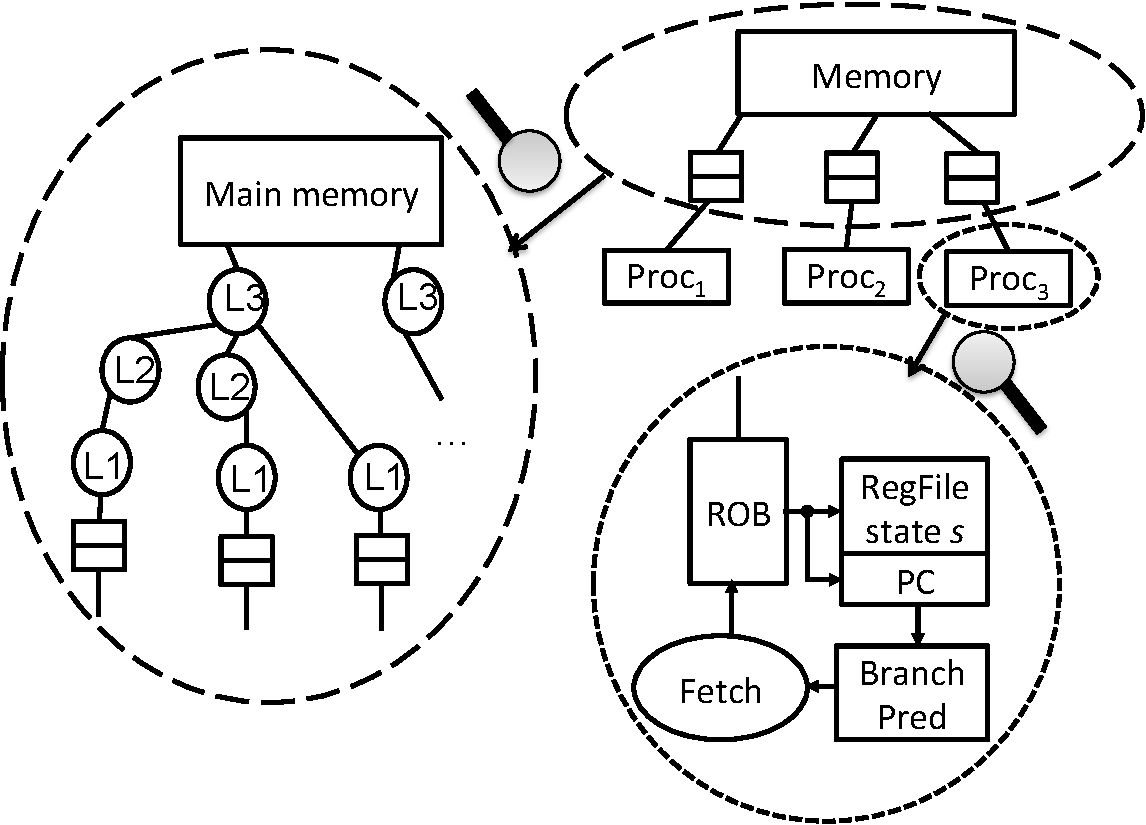
\includegraphics[scale=.43]{zoom}
%\caption{Overall system}
%\label{zoom}
%\end{figure}
%
%Figure \ref{zoom} sketches the sort of hardware system that we have verified.
%We show the top-level system design at top right, and we zoom in on boxes standing for the
%memory system and a single processor.
%
%Memory is composed of a \emph{hierarchy of caches}, where each cache node (labeled
%like ``L1,'' ``L2,'' etc.) communicates only with its neighbors in the graph.
%Each processor has a dedicated L1 cache, from which we do our best to satisfy
%all memory requests, to avoid the latency of a round-trip with main memory.
%With an L1 cache miss, we may still find a hit in a parent cache below the
%level of main memory, realizing a smaller but still significant speedup.
%We have verified a \emph{directory-based} protocol for coordinating an arbitrary
%tree of caches, where each node stores a conservative approximation of its
%children's states.
%
%A processor is decomposed into several components.  We have the normal
%architectural state, such as values of registers.  Our proofs are generic over
%\emph{a family of instruction set architectures}, with parameters for opcode sets and
%functions for executing opcodes and decoding them from memory.  Other key
%components are a \emph{branch predictor}, which guesses at the control-flow path
%that a processor will follow, to facilitate speculation; and a
%\emph{reorder buffer (ROB)}, which decides which instructions along that path to
%try executing ahead of schedule.  Our proofs apply to an arbitrary branch predictor,
%and they work for any reorder buffer satisfying a simple semantic condition.
%
%Figure~\ref{proofs} gives the overall proof structure that we employ to verify
%the system of Figure~\ref{zoom}. As we will explain later, $P_\text{so}$
%represents the speculative out-of-order processor, $M_c$ the cache memory,
%$M_m$ the simple memory, $P_\text{ref}$ a simple decoupled processor, and
%SC the simple reference model having multiple processors executing each
%instruction atomically thus implementing sequential consistency.  Notation
%$A^n$ is for $n$ copies of system $A$ running in parallel.
%$\sqsubseteq$ is a refinement operator, capturing a suitable notion of when
%one system implements another.  We go into more detail on the symbols from
%the figure in the rest of the paper.
%
%Our current framework establishes theorems of the form ``if system $A$ has a run
%with some particular observable behavior, then system $B$ also has a run with
%the same behavior.''  In this sense, we say that $A$ correctly implements $B$.
%Other important properties, such as \emph{deadlock freedom} for $A$ (which
%might get stuck without producing any useful behavior), we leave for future
%work.
%
%\begin{figure}
%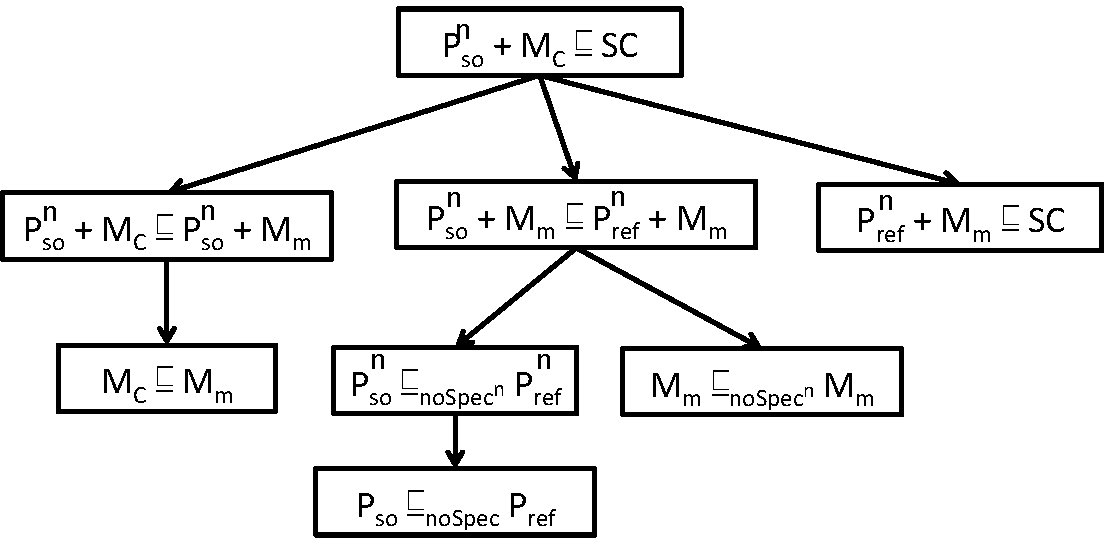
\includegraphics[scale=.45]{proofs}
%\caption{Overall proof structure}
%\label{proofs}
%\end{figure}


%% Modularity has long been understood as a key property for effective design and
%% verification of complex systems, \eg\ distributed memory systems. For the
%% designer, it allows a separation of concerns increasing robustness by allowing
%% the behavior encapsulated by a modular boundary to be realized by multiple
%% implementation any of which may be safely dropped into the system. It also
%% allows a greater measure of parallelization of design improving development
%% time. Similarly verification is simplified as modular interface agreements
%% provide a set of natural lemmas to verify. This leads us towards a
%% decomposition of the whole system verification task into smaller more
%% manageable chunks.

%% Given its complexity, it is a practical necessity for distributed shared memory
%% systems to be built a strong idea of modularity. The standard modularization
%% (see Figure~\ref{fig:highleveldsm}) separates the ISA-level processors nodes
%% which are responsible for executing threads of computation, and a unified
%% shared memory subsystem which is responsible for ensuring that memory requests
%% it receives are handled correctly, \ie{} in line with the memory model which
%% dictates which store values a load may observe in the system. These processors
%% may then be refined for performance, while the monolithic memory module is
%% improved by introducing layers of caching and a coherence protocol to guarantee
%% memory consistency.

%% This high-level approaches works reasonably well for implementation; separate
%% design groups tackle can each task in isolation. However, when we consider
%% verification, the modularity enforced during the implementation has little
%% benefit and in practice we must resort to full system verification. The core of
%% this problem lies in the fact that the simple high-level decomposition of
%% memory and processors does not fully take into account the space of speculation
%% techniques used in the processor.

%% All practical processor instruction set architectures (ISAs) are fairly
%% sequential; the result of executing an instruction may affect which next
%% instruction is executed. As a result for performance some sort of prediction is
%% used to allow instructions to be speculatively started and executed before the
%% previous instructions have completed and the values need to execute are known.
%% Additional bookkeeping is used to determine when our guess is wrong and
%% false-path instructions are undone leaving no affect on the architectural
%% state. As precise exception handling is a requirement these speculative
%% instructions are committed, \ie{} expose their effects of execution to the
%% whole system, in sequence.

%% Though most forms of speculation (\eg{} branch prediction, instruction prefetch
%% from pipelining, value prediction) are often considered as being orthogonal to
%% memory issues, speculation changes the sequence of memory requests the
%% processor sends to the memory. This may be merely handling requests out of
%% order, \eg{} issuing a load request before a logically earlier one has issued
%% (a common occurrence due to data dependencies in out-of-order processors). We
%% may also allow incorrect memory operations to be issued, \eg{} executing a load
%% from a false path. It is worth noting that while such load operations are
%% possible to speculate, we cannot speculatively issues store operations to the
%% memory as they become exposed to the whole system and speculation mechanisms
%% are isolated to a single processor. As a consequence of this, our memory does
%% not know what order requests it is sent should happen. Thus the memory in
%% isolation cannot directly realize the memory model and in actually implements a
%% much weaker model leaving the full enforcement of the memory model to the
%% processor which can enforce this by restricting when it issues requests. 

%% The goal of this work is to introduce an interface enabling true modular
%% implementation and verification of shared memory systems. That is, we should be
%% able to describe a modular decomposition where we may correct replace either
%% the processor nodes, the memory with locally verified alternatives without
%% changing the correctness of our whole system proof of correctness or
%% restricting our ability to describe shared memory systems. As part of this we
%% will describe the processor interface in a way which allows the full range of speculation 

%% We do so by showing the construction and initial refinements of a sequentially
%% consistent shared memory system. We formally defining a minimal cache coherent
%% speculation-friendly memory interface (\emph{Store Atomicity}), and use this as
%% the interface for our memory subsystem. Using this we specify the notion of
%% correct for a processor and prove that our system is correct assuming the
%% correct implementation of these two objects.  We then construct both a naive
%% reference processor and memory subsystem and provide proofs of correctness in
%% Coq. We then refine both components into more realistic implementations
%% including taking our memory subsystem to hardware-level description of a
%% arbitrary-level hierarchical cache coherence implementation and verify these
%% module. We show that the cross products of possible implementations are correct
%% and their proof automatically from the modularly.

%%  LocalWords:  Modularity modularity

%\section{Defining Sequential Consistency}

To dicsuss the modularization of our system we must first fully define what we
mean by sequential consistency. Informally, sequential consistency states that
the memory operations from all processors in the system are evaluated
atomically with regards to each other by the memory and are evaluated in order
locally but with no ordering requirements between operations from different
processors.

Formally Sequential Consistency can be described as:

\xxx{SC Definition HERE}. 

\xxx{TOTAL ORDERING CONDITION} 

Total ordering is not generally stated. 





%\section{Enabling Practical Memory Subsystems: Atomic Store}

The behavior of a memory system realizing different memory models or
interfacing with different levels speculation from the processors would be
dramatically different. For instance, a memory system realizing Total Store
Order allows significantly the more memory requests to be in flight than in a
sequential consistent system. As such one might expect that there should be
relatively little sharing between designs.




%% At a high-level, the physical interface of memory is fairly consistent
%% regardless of the memory model or instruction execution scheme. The processor
%% makes requests (loads and stores) and gets responses back from the
%% memory. 


Memory subsystems are designed to allow parallel operation 

The most natural interface for a memory subsystem is to expect the interface to 



Memory needs caches, highly pipelined. All worries happen at a single address. No ordering guarantees between two different addresses. This is a natural representation because. 

Clearly this model is not SC. However, it is highly atuned to high-performance results.

%\section{How to Build and Sequentially System using Atomic Store}

We can have a simple system using a lamport-like processor which will nopipelining of memory. Trivially SC with atomic store. This is obviously correct, but from a point of view of practice, we must pipeline this. We need to refine this model into a

(How to use a non-monolithic memory).

\section{How to build a monolithic processor}

A speculative Lamport system consists of a monolithic memory and other loads and stores. This is how this system works. Need to discuss 

* need definitions of spec processor. (Must be complete and sound)

A full realistic implementation:



\section{Labeled Transition Systems}\label{sec:lts}

We make extensive use of the general theory of labeled transition
systems, a semantics approach especially relevant to communicating
concurrent systems.  As we are formalizing processors for
Turing-complete machine languages, it is challenging to prove that a
system preserves almost any aspect of processor behavior from a model
like SC.  To focus our theorems, we pick the time-honored property of
\emph{termination}.  An optimized system should terminate or diverge
iff the reference system could also terminate or diverge,
respectively.  Our basic definitions of transition systems build in
special treatment of halting, so that we need not mention it
explicitly in most contexts to come.

\begin{defn}
A \textbf{labeled transition system (LTS)} is a ternary relation, over
$\mathcal S^H \times \mathcal L^\epsilon \times \mathcal S^H$, for some sets
$\mathcal S$ of states and $\mathcal L$ of labels. We usually do not mention
these sets explicitly, as they tend to be clear from context. We write
$X^\epsilon$ for lifting of a set $X$ to have an extra ``empty'' element
$\epsilon$ (like an \texttt{option} type in ML). We write $X^H$ for lifting of
a set $X$ to have an extra ``halt'' element $H$. We also implicitly consider
each LTS to be associated with an \emph{initial} state in $\mathcal S$.
\end{defn}

For LTS $A$, we write $\io{A}{s}{s'}{\ell}$ as shorthand for $(s,
\ell, s') \in A$, and we write $A_0$ for $A$'s initial state. The
intuition is that $A$ is one process within a concurrent system. The
label $\ell$ from set $\mathcal L$ of labels is produced when $A$
participates in some IO exchange with another process; otherwise it is
an empty or ``silent'' label $\epsilon$.  As a shorthand, we sometimes
omit labels for $\epsilon$ steps.  Note that the IO exchange can be
input, output, or both, and its interpretation is dependent on the
context.


\subsection{Basic Constructions on LTSes}

From an LTS representing single-step system evolution, we often want to build
an LTS capturing arbitrary-length evolutions.

\begin{defn}
The \textbf{transitive-reflexive closure} of $A$, written $A^{*}$, is a derived
LTS.  Where $A$'s states and labels are $\mathcal S$ and $\mathcal L$, the
states of $A^{*}$ are $\mathcal S$, and the labels are $\mathcal L^{*}$, or
\emph{sequences} of labels from the original system.  $A^{*}$ steps from $s$ to
$s'$ when there exist zero or more transitions in $A$ that move from $s$ to
$s'$.  The label of this transition is the \emph{concatenation} of all labels
generated in $A$, where the empty or ``silent'' label $\epsilon$ is treated as
an identity element for concatenation.
\end{defn}

We also want to compose $n$ copies of an LTS together, with no explicit
communication between them.  We apply this construction later to lift a
single-CPU system to a multi-CPU system.

\begin{defn}
The \textbf{$n$-repetition} of $A$, written $\smulti{n}{A}$, is a derived LTS.
Where $A$'s states and labels are $\mathcal S$ and $\mathcal L$, the states of
$\smulti{n}{A}$ are $\mathcal S^n$, and the labels are $[1, n] \times \mathcal
L$, or pairs that \emph{tag} labels with which component system generated them.
These labels are generated only when the component system generates a label.
The whole system halts whenever one of the components halts.  We define the
transition relation with the following inference rules. We treat $n$-tuples as
functions keyed on numeric positions, and we write $\theta[i := v]$ for
updating $n$-tuple $\theta$ to overwrite the $i$th position with value $v$, and
we treat any label $(i, \epsilon)$ as $\epsilon$.
$$\inference[i]
{\theta(i) = a & \io{$A$}{a}{a'}{\ell} & a' \neq H}
{\io{$\smulti{n}{A}$}{\theta}{\theta[i:=a']}{i,\ell}}
\quad \inference[H]
{\io{$A$}{\theta(i)}{H}{\ell}}
{\io{$\smulti{n}{A}$}{\theta}{H}{i,\ell}}
$$
\end{defn}

Eventually, we need processes to be able to communicate with each
other, which we formalize via the $+$ composition operator. It
connects same-label transitions in the two systems, treating the label
as a cooperative communication event that may now be hidden from the
outside world, as an $\epsilon$ label.

\begin{defn}\label{plus}
Where $A$ and $B$ are two LTSes sharing labels set $\mathcal L$,
and with state sets $\mathcal S_A$ and
$\mathcal S_B$ respectively, the \textbf{communicating composition} $A + B$ is
a new LTS with states $\mathcal S_A \times \mathcal S_B$ and an empty label set,
defined as follows:
\vspace{-.2in}\begin{center}
$$\inference[$A$]
{\io{$A$}{a}{a'}{} & a' \neq H}
{\io{$A + B$}{a, b}{a', b}{}}
\quad \inference[$B$]
{\io{$B$}{b}{b'}{} & b' \neq H}
{\io{$A + B$}{a, b}{a, b'}{}}$$
$$\inference[H$_A$]
{\io{$A$}{a}{H}{}}
{\io{$A + B$}{a, b}{H}{}}
\quad \inference[H$_B$]
{\io{$B$}{b}{H}{}}
{\io{$A + B$}{a, b}{H}{}}$$
$$\inference[Join]
{\io{$A$}{a}{a'}{\ell} & \io{$B$}{b}{b'}{\ell} & a', b' \neq H}
{\io{$A + B$}{a, b}{a', b'}{}}$$
\end{center}
\end{defn}

\subsection{Refinement Between LTSes}

We need a notion of when one LTS ``implements'' another.  Intuitively,
transition labels and halting are all that the outside world
can observe. Two systems that produce identical labels and termination behavior
under all circumstances can be considered as safe substitutes for
one another. We will only need an asymmetrical notion of compatibility:

\begin{defn}\label{refines}
For some label domain $\mathcal L$, let $f : \mathcal L \to \mathcal L^\epsilon$ 
be a function that is able to replace labels with alternative
labels, or erase them altogether. Let LTSes $A$ and $B$ have the same label
set $\mathcal L$. We say that
\textbf{$A$ trace-refines $B$ w.r.t. $f$}, or $A \sqsubseteq_f B$, if:
\begin{multline*}
\forall s_A, \eta. \; \io{$A^{*}$}{A_0}{s_A}{\eta} \Rightarrow \exists s_B. \;
\io{$B^{*}$}{B_0}{s_B}{f(\eta)} \; \wedge \\
(s_A = H \Leftrightarrow s_B = H)
\end{multline*}
Each label in the trace is replaced by the mapping of $f$ on it, and
labels mapped to $\epsilon$ by $f$ are dropped. $f$ is overloaded
to denote that multi-label version when applied to $\eta$.
\end{defn}

As a shorthand, we write $A \sqsubseteq B$ for $A \sqsubseteq_\mathsf{id} B$,
for $\mathsf{id}$ an identity function, forcing traces in the two systems to
match exactly. Under this notion of identical traces, we say that $A$
is sound w.r.t. $B$.

\subsection{A Few Useful Lemmas}

The reflexivity and transitivity properties of refinement are crucial to help us
structure modular proofs.

\begin{theorem}\label{transitive}
$\sqsubseteq$ is reflexive and transitive.
\end{theorem}

Another crucial proof step is to lift a single-process result to the $n$-way
replication of that process.

\begin{theorem}\label{liftn}
If $A \sqsubseteq_f B$, then $\smulti{n}{A} \sqsubseteq_{f^n} \smulti{n}{B}$, where
$f^n$ is $f$ lifted appropriately to deal with indices ($f^n(i, \ell) =
(i, \ell')$ when $f(\ell) = \ell'$, and $f^n(i, \ell) = \epsilon$ when
$f(\ell) = \epsilon$).
\end{theorem}

We will also need a result applying to communicating compositions.

\begin{theorem}\label{liftplus}
If $A \sqsubseteq_f A'$ and $B \sqsubseteq_f B'$, then $A + B \sqsubseteq A' +
B'$. In other words, if systems $A$ and $B$ are individually simulated by $A'$ and
$B'$ on identical alteration of the traces, then the composed
system $A+B$ will be sound with respect to $A'+B'$.
\end{theorem}

\begin{figure}
\small
\centering
\begin{boxedminipage}[c]{.48\textwidth}
%\centering
\inference
[Halt]
{\theta(i) = (s, \pc) & \dec(s,\pc) = H}
{\io{SC}{\theta,m}{H}{}}

\inference
[NonMem]
{\theta(i) = (s, \pc) & \dec(s,\pc) = (\nm, x) \\ \exec(s, \pc, (\nm, x)) = (\pc', s')}
{\io{SC}{\theta,m}{\theta[i \coloneqq (s', \pc')], m}{}}

\inference
[Load]
{\theta(i) = (s,\pc) & \dec(s,\pc) = (\ld, x, a) \\ \exec(s, \pc, (\ld, x, m(a))) = (\pc', s')}
{\io{SC}{\theta,m}{\theta[i\coloneqq(s',\pc')],m}{}}

\inference
[Store]
{\theta(i) = (s,\pc) & \dec(s,\pc) = (\st, a, v) \\ \exec(s, \pc, (\st)) = (\pc', s')}
{\io{SC}{\theta,m}{\theta[i\coloneqq(s',\pc')],m[a\coloneqq v]}{}}
\end{boxedminipage}
\caption{LTS for sequential consistency with $n$ simple processors}
\label{Ref}
\end{figure}

\section{Decomposing a Multi-Processor System}
\label{sec:store-atomicity}

\begin{figure}
\centering
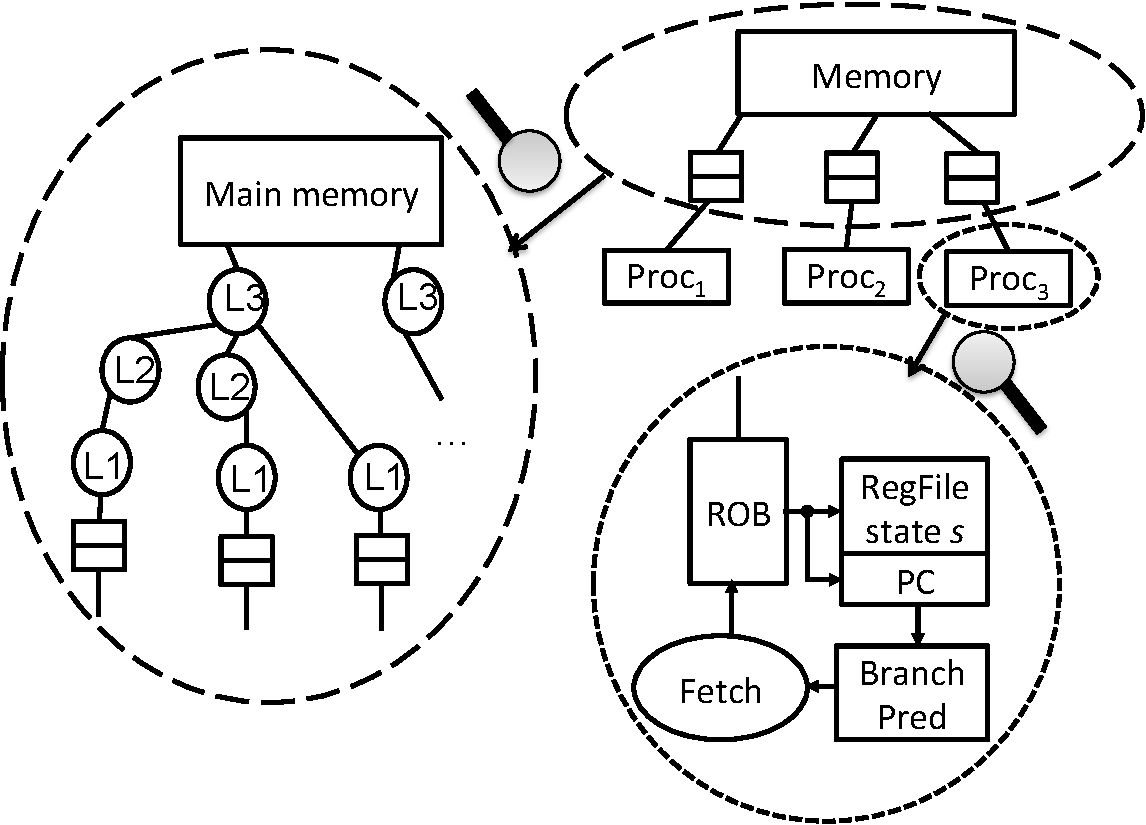
\includegraphics[scale=.43]{zoom}
\caption{Components of a multi-processors system}
\label{zoom}
\end{figure}

Most any conventional multi-processor system can be divided into 3 components as shown in
Figure \ref{zoom}. 
We show the top-level system design at top right, and we zoom in on boxes standing for the
memory system and a single processor ($P_i$).
The processor component $P_i$ can be implemented in a
variety of ways, from literal execution of instructions in program order, to complex speculation
with instructions run simultaneously to exploit parallelism. The memory component is normally implemented
using a hierarchy of caches, in order to increase the performance of the
overall system, since the latency of accessing a memory directly is very slow
compared to accessing a much smaller cache. The component between each
processor and the global memory sub-system contains local buffers, $B_i$, specific to
the processor $P_i$ they are connected to. 

\begin{figure}
\small
\centering
\begin{boxedminipage}[c]{.48\textwidth}
\inference
[Load]
{}
{\io{$M_m$}{m}{m}{(\ld\req,a),(\ld\resp,m(a))}}

\inference
[Store]
{}
{\io{$M_m$}{m}{m[a\coloneqq v]}{(\st, a, v)}}

\end{boxedminipage}
\caption{LTS for a simple memory}
\label{$M_m$}
\end{figure}

Popular instruction set architectures do not guarantee sequential
consistency.  That is, their behavior makes it unsound to imagine that
the different processors of a shared-memory system are running
according to simple interleaving, where each instruction executes
atomically.  However, we want to emphasize that, in every weak-memory
system we are aware of, \emph{the main memory still exposes atomic
  loads and stores}!  The weaker semantics arises only because of (1)
reordering of memory instructions by the core $P_i$ and/or (2) the
properties of the local buffers $B_i$ connected to each processor
$P_i$.  For instance, if $B_i$ were a store buffer, into which the
committed stores from an in-order processor $P_i$ are enqueued, and if
any ``subsequent'' load from the same processor $P_i$ reads the latest
value from the store buffer, then one can establish that such a
multi-processor system implements the TSO~\cite{x86tsocacm10} memory
model.

So, we focus on this opportunity to simplify proof decomposition.  We
will prove that our main memory component satisfies an intuitive
\emph{store atomicity} property.  Despite the potential red herring of
the word ``atomicity,'' this specification is appropriate even for
implementation of weaker memory models than SC.  Store atomicity can
be understood via the operational semantics of Figure \ref{$M_m$},
describing an LTS that receives load and store requests ($\ld$ and
$\st$) from processors and sends back load responses ($\ld\resp$).

The memory component is composed of a \emph{hierarchy of caches}, where each
cache node (labeled like ``L1,'' ``L2,'' etc.) communicates only with its
neighbors in the graph.  Each processor has a dedicated L1 cache, from which we
do our best to satisfy all memory requests, to avoid the latency of a
round-trip with main memory.  With an L1 cache miss, we may still find a hit in
a parent cache below the level of main memory, realizing a smaller but still
significant speedup.  Therefore it is the responsibility of the hierarchy of
caches, which forms the memory sub-component, to implement the store atomicity
property. In fact, as we will prove in Section \ref{sec:cc}, the purpose of the
cache-coherence protocol is to establish this invariant for the memory
sub-component.  Concretely, we have verified a \emph{directory-based} protocol
for coordinating an arbitrary tree of caches, where each node stores a
conservative approximation of its children's states.

As an instance of the above decomposition, we will prove that a multi-processor
system with no local buffering in between the processor and the memory
components indeed implements sequential consistency. We implement a highly
speculative processor that executes instructions and issues loads out of
order, but commits instructions (once some ``verification'' is done) in order.

The processor itself can be decomposed into several components. In the zoomed-in
version of Figure \ref{zoom}, we show a highly speculative, out-of-order
issue processor. We have the normal architectural state, such as values of
registers.  Our proofs are generic over \emph{a family of instruction set
architectures}, with parameters for opcode sets and functions for executing
opcodes and decoding them from memory.  Other key components are a \emph{branch
predictor}, which guesses at the control-flow path that a processor will
follow, to facilitate speculation; and a \emph{reorder buffer (ROB)}, which
decides which instructions along that path to try executing ahead of schedule.
Our proofs apply to an arbitrary branch predictor, and they work for any
reorder buffer satisfying a simple semantic condition.

Figure~\ref{proofs} gives the overall proof structure that we employ to verify
the system of Figure~\ref{zoom}. As we will explain later, $P_\text{so}$
represents the speculative out-of-order processor, $M_c$ the cache memory,
$M_m$ the simple memory, $P_\text{ref}$ a simple decoupled processor, and
SC the simple composition of P$^n_\text{ref}+ M_m$ executing each
instruction atomically, thus implementing sequential consistency.

Our current framework establishes theorems of the form ``if system $A$ has a run
with some particular observable behavior, then system $B$ also has a run with
the same behavior.''  In this sense, we say that $A$ correctly implements $B$.
Other important properties, such as \emph{deadlock freedom} for $A$ (which
might get stuck without producing any useful behavior), we leave for future
work.

\begin{figure}
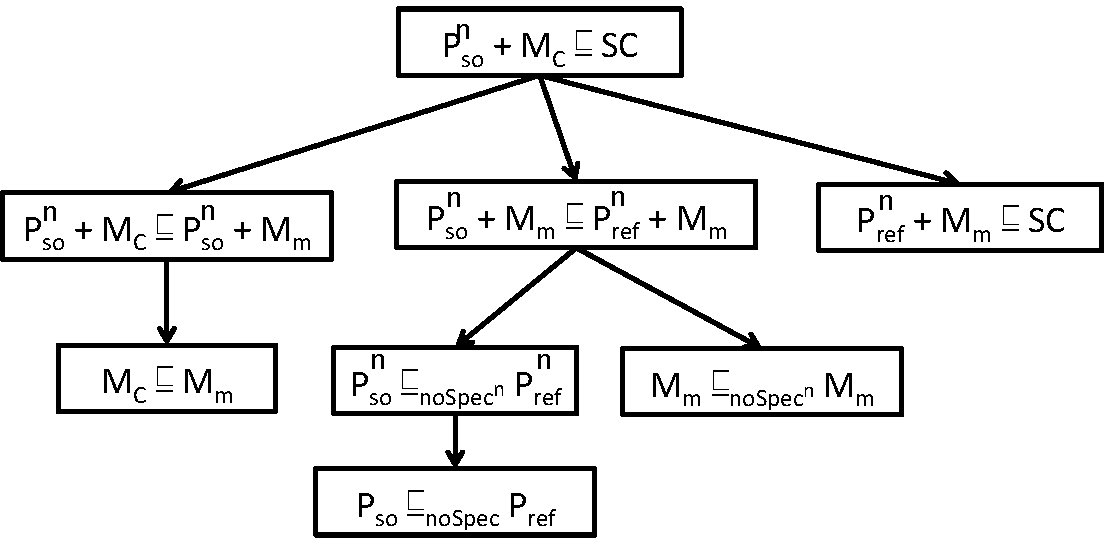
\includegraphics[scale=.45]{proofs}
\caption{Overall proof structure}
\label{proofs}
\end{figure}

\section{Specifying Sequential Consistency}\label{sec:sc}

Our final theorem in this paper establishes that a particular complex hardware
system implements sequential consistency (SC) properly.  We state the theorem
in terms of the trace refinement relation $\sqsubseteq$.
Therefore, we need to define an LTS embodying SC.  The simpler this
system, the better.  We do not need to worry about its performance properties,
since we will prove that an optimized system remains faithful to it.

\begin{figure}
\small
\centering
\begin{boxedminipage}[c]{.48\textwidth}
\inference
[Halt]
{\dec(s,\pc) = H}
{\io{P$_\text{ref}$}{s,\pc}{H}{}}

\inference
[NM]
{\dec(s,\pc) = (\nm, x) & \exec(s, \pc, (\nm, x)) = (\pc', s')}
{\ioe{P$_\text{ref}$}{s,\pc}{s', \pc'}}

\inference
[Ld]
{\dec(s,\pc) = (\ld, x, a) & \exec(s, \pc, (\ld, x, v)) = (\pc', s')}
{\io{P$_\text{ref}$}{s, \pc}
{s', \pc'}{(\ld\req, a), (\ld\resp, v)}}

\inference
[St]
{\dec(s,\pc) = (\st, a, v) & \exec(s, \pc, (\st)) = (\pc', s')}
{\io{P$_\text{ref}$}{s, \pc}
{s', \pc'}{(\st, a, v)}}
\end{boxedminipage}

\caption{LTS for a single reference processor (P$_{\text{ref}}$)}
\label{Pref$}
\end{figure}


Figure \ref{Pref$} shows the LTS for a single processor that will be used as a
reference processor.  The definition is parametrized over details of an
\emph{instruction set architecture} (ISA).  In particular, the ISA gives us
some domains of architectural states $s$ (e.g., register files) and of program
counters $\pc$.  A function $\dec(s, \pc)$ figures out which instruction $\pc$
references in the current state, returning the instruction's ``decoded'' form.
A companion function $\exec(s, \pc, \mathit{dec})$ actually executes the
instruction, returning the next program counter $\pc'$ and the new state $s'$.

The legal instruction forms, which are outputs of $\dec$, are $(\nm, x)$, for
an operation not accessing memory; $(\ld, x, a)$, for a memory load from
address $a$; $(\st, a, v)$, for a memory store of value $v$ to address $a$; and
$H$, for a ``halt'' instruction that moves the LTS to state $H$. The parameter
$x$ above represents the rest of the instruction, including the
opcode, registers, constants, \etc{}

The legal inputs to $\exec$ encode both a decoded instruction and any relevant
responses from the memory system.  These inputs are $(\nm, x)$ and $\st$, which
need no extra input from the memory; and $(\ld, x, v)$, where $v$ gives the
contents of the requested memory cell.

We can define sequential consistency using the simple memory from Figure
\ref{$M_m$} as follows, for $n$ processors:
\begin{defn}
$SC \triangleq P^n_\text{ref} + M_m$
\label{sc}
\end{defn}

We define the initial state of SC as $(\theta_0, m_0)$, where $m_0$ is
some initial memory fixed throughout our development, mapping every
address to value $v_0$; and $\theta_0$ maps every processor ID to
$(s_0, \pc_0)$, using architecture-specific default values $s_0$ and
$\pc_0$.

This LTS encodes Lamport's notion of SC, where processors take turns executing
nondeterministically in a simple interleaving.  We need know very few details
of the ISA to define the SC model.  Our final, optimized system is parametrized
over an ISA in the same way.  In the course of the rest of this paper, we will
define an optimized system $O$ and prove $O \sqsubseteq \text{SC}$.

Note that, in this setting, an operational specification like the LTS
for SC is precisely the right characterization of \textbf{full functional
  correctness} for a hardware design, much as a
precondition-postcondition pair does that job in a partial-correctness
Hoare logic.  Our SC LTS fully constrains observable behavior of a
system to remain consistent with simple interleaving.  Similar
operational models are possible as top-level specifications for
systems following weaker memory models.


\section{Speculative Out-Of-Order Processor}\label{sec:ooo}

The previous section divided a multiprocessor system into two rather
simple components, processors and memories.  We are now ready to begin
developing more complex, optimized versions of each piece, starting
with processors.

We implement a \emph{speculative} processor, which may create many
simultaneous outstanding requests to the memory, as an optimization to
increase parallelism.  Our processor proof is in some sense generic
over correct speculation strategies.  We parametrize over two key
components of a processor design: a \emph{branch predictor}, which
makes guesses about processor-local control flow in advance of
%receiving enough memory responses to resolve
resolving conditional jumps; and a
\emph{reorder buffer}, which decides what speculative instructions (like memory loads)
are worth issuing at which moments (in effect \emph{reordering} later
instructions to happen before earlier instructions have finished).

The branch predictor is the simpler of the two components to model.
We indicate branch-predictor state with metavariable $\ppc$.
The operations on such state are $\curPpc(\ppc)$, to extract the
current program-counter prediction; $\nextPpc(\ppc)$, to ask the
predictor to step forward by one instruction; and $\setBp(\ppc, \pc)$,
to reset prediction to begin at a known-accurate position $\pc$.  It
turns out that we need to impose no explicit correctness criterion on
branch predictors.  The processor uses predictions only as hints, and
it always resets the predictor using $\setBp$ after detecting an
inaccurate hint.

The interface and formal contract of a reorder buffer are more
involved.  We write $\rob$ as a metavariable for reorder buffer
state.  The associated operations are:
\begin{itemize}
\item $\phi$, the state of an empty buffer.
\item $\add(\pc, \rob)$, which appends the program instruction at location $\pc$ to the list of instructions that the buffer is allowed to consider executing.
\item $\get\spc\ld(\rob)$, which returns an optional speculative load to issue
\item $\compute(\rob)$, which models a
step of computation inside the buffer. For instance, it invokes the $\dec$
and $\exec$ functions (as defined for SC) internally to obtain the next program
counter, state, \etc{} (only the speculative states are updated, not the actual states).
\item $\upd\ld(\rob,t,v)$, which informs the buffer that the memory
has returned result value $v$ for the speculative load with tag $t$.
\item $\commit(\rob)$, which returns the next instruction in serial
program order, if we have accumulated enough memory responses to execute it
accurately, or returns
$\epsilon$ otherwise.  When $\commit$ returns an instruction, it also
returns the associated program counter plus the next program counter
we would advance to afterward.
 Furthermore, the instruction is
extended with any relevant response from memory (used only for load
instructions, obtained through $\upd\ld$) and with the new architectural state (\eg{} register
file) after execution.
\item $\retire(\rob)$, which informs the buffer that its $\commit$
instruction was executed successfully, so it is time to move on to the
next instruction.
\end{itemize}

We postpone characterization of correct reorder buffers until after we
present the LTS for speculating processors.

\begin{figure*}[t]
\small
\centering
\begin{boxedminipage}[c]{.95\textwidth}
\inference[Fetch]
{}
{\ioe{P$_\text{so}$}{s,\pc,\rob,\ppc}{s,\pc,\add(\curPpc(\ppc),\rob),\nextPpc(\ppc)}}

\inference[Compute]
{\get\spc\ld(\rob) = \epsilon}
{\ioe{\text{P$_\text{so}$}}{s,\pc,\rob,\ppc}{s,\pc,\compute(\rob),\ppc}}

\inference[SpecLd]
{\get\spc\ld(\rob) = (\spc\ld,t,a)}
{\io{\text{P$_\text{so}$}}{s,\pc,\rob,\ppc}{s,\pc,\upd\ld(\compute(\rob),t,v),\ppc}
{(\ld\req, a), (\ld\resp, v)}}


\inference[Abort]
{\commit(\rob) = (\pc',\_,\_) & \pc' \neq \pc}
{\ioe{\text{P$_\text{so}$}}{s,\pc,\rob,\ppc}{s,\pc,\phi,\setBp(\ppc,\pc)}}

\inference[Halt]
{\commit(\rob) = H}
{\ioe{\text{P$_\text{so}$}}{s,\pc,\rob,\ppc}{H}}

\inference[Nm]
{\commit(\rob) = (\pc,\pc',(\nm,s'))}
{\ioe{\text{P$_\text{so}$}}{s,\pc,\rob,\ppc}{s',\pc',\retire(\rob),\ppc}}

\inference[St]
{\commit(\rob) = (\pc,\pc',(\st,a,v,s'))}
{\io{\text{P$_\text{so}$}}{s',\pc',\retire(\rob),\ppc}{s,\pc,\rob,\ppc}
{\st, a, v}}

\inference[LdGood]
{\commit(\rob) = (\pc,\pc',(\ld,x,a,v,s'))}
{\io{\text{P$_\text{so}$}}{s,\pc,\rob,\ppc}{s',\pc',\retire(\rob),\ppc}{(\ld\req, a), (\ld\resp, v)}}

\inference[LdBad]
{\commit(\rob) = (\pc,\pc',(\ld,x,a,v',s')) & v' \neq v & \exec(s,\pc,(\ld,x,v)) = (\pc'', s'')}
{\io{\text{P$_\text{so}$}}{s,\pc,\rob,\ppc}{s'',\pc'',\phi,\setBp(\ppc,\pc)}{(\ld\req, v), (\ld\resp,v)}}
\end{boxedminipage}

\caption{Speculating, out-of-order issue processor}
\label{Ooo}
\end{figure*}

Figure~\ref{Ooo} defines that LTS,
P$_{\texttt{so}}$. This processor may issue arbitrary speculative
loads, but it only ever \emph{commits} the next instruction in serial
program order. 
We will see the processor issue two kinds of loads, a speculative
load ($\spc\ld$) and a commit or real load ($\ld$).  To maintain SC, every speculative
load must have a matching verification load later on, and we maintain
the illusion that the program only depends on the results of
verification loads, which, along with stores, \emph{must be issued in
serial program order}.

When committing a
previously issued speculative load instruction, the associated speculative
memory load response is verified against the new commit load response. If the
resulting values do not match, the processor terminates all past uncommitted
speculation, by emptying the reorder buffer and resetting the
next predicted program counter in the branch predictor to the correct next value. This step mimics
the mechanism implemented in most modern-day processors, operating on the
conservative assumption that the processor may have performed arbitrary
incorrect speculation after receiving the inaccurate response from
memory.  (Note that here ``inaccurate'' does not mean ``wrong at
the time the response was received,'' but rather ``wrong at commit
time'' or ``correct before, but not anymore.'')

A full processor state is $(s, \pc, \rob, \ppc)$, comprising
architectural state, the program counter, and the reorder buffer and branch
predictor states. Its initial state is given by $(s_0, \pc_0, \phi, \ppc_0)$.
The interface of this processor with memory is identical
to that of the reference processor, but now we can exercise a memory
system's transitions even for speculative loads.

\begin{figure*}[t]
\small
\begin{inv}
If $P_\text{so}$ reaches a state $(s, \pc, \rob, \ppc)$, \ie{}

$\io{P$_\text{so}^{*}$}{s_0,\pc_0,\phi,\ppc_0}{s,\pc,\rob,\ppc}{\eta} \Rightarrow$
\begin{displaymath}
\left\{
\begin{array}{ll}
\commit(\rob) = (\pc, \pc', (\nm, s')) &\Rightarrow
\exists x. \; \dec(s,\pc) = (\nm, x) \wedge \exec(s,\pc, (\nm,x)) =
(\pc', s')\\
\commit(\rob) = (\pc, \pc', (\ld, x, a, v, s')) & \Rightarrow
\dec(s,\pc) = (\ld, x,a) \wedge \exec(s,\pc, (\ld,x,v)) = (\pc', s')\\
\commit(\rob) = (\pc, \pc', (\st, a, v, s')) &\Rightarrow
\dec(s,\pc) = (\st, a,v) \wedge \exec(s,\pc, (\st)) =
(\pc', s')\\
\commit(\rob) = H & \Rightarrow
\dec(s, \pc) = H\\
\end{array}
\right.\end{displaymath}
\label{rob}
\end{inv}
\vspace{-.5cm}
\caption{Correctness of reorder buffer}
\label{robfig}
\end{figure*}

Finally, we impose a general correctness condition on reorder
buffers.  They must maintain Invariant~\ref{rob} in Figure~\ref{robfig}.
Intuitively, whenever the buffer claims in a $\commit$
output that a particular instruction is next to execute, causing
certain state changes, that instruction must really be next in line according
to how the program runs in the SC system, and running it must really cause
those state changes.

When this condition holds, we may conclude the correctness theorem for
out-of-order processors.  We use a trace-transformation function
$\noSpec$ that drops all speculative-load requests and responses.
See Definition~\ref{refines} for a review of how we use such
functions in framing trace refinement.  Intuitively, we prove that any
behavior by the speculating processor can be matched by the simple
processor, with speculative messages erased.

\begin{theorem}
\label{ocorrect}
$\text{P$_\text{so}$} \sqsubseteq_\noSpec$ P$_\text{ref}$
\end{theorem}
\begin{proof}
By induction on P$_\text{so}$ traces, using a proper abstraction
function (which drops the speculative messages and the $\rob$ and $\ppc$ states) to relate the two systems.  Invariant~\ref{rob} is crucial to
relate the reorder buffer's behavior with the simple in-order
execution of P$_\text{ref}$.
\end{proof}

\begin{corollary}
\label{ges}
$\text{P$^n_\text{so}$} \sqsubseteq_{\noSpec^n}$ P$_\text{ref}^n$
\end{corollary}
\begin{proof}
Direct consequence of Theorems~\ref{ocorrect} and~\ref{liftn} (where the
latter is one of our preliminary results about $n$-repetition).
\end{proof}


\section{Cache-Based Memory System}\label{sec:cc}

We now turn our attention toward a more efficient implementation of
memory.  It is physically infeasible to connect many processors
directly to a single memory with low enough latency to handle most
memory requests quickly enough.  Instead, each processor will have its
own \emph{L1 cache} of recently used memory cells.  Whenever possible, we
want to service memory requests from processors' own caches, only
contacting memory for addresses not found in the caches.  To further
avoid contacting main memory, we create additional higher-level
caches, connecting each L1 cache to an L2 cache, potentially
connecting L2 caches to L3, etc., bottoming out in main memory at the
root of our tree. The zoomed-in portion of the memory in Figure~\ref{zoom}
diagrams the basic layout.

Now we have concurrent interaction of many processors with many caches
with main memory, and the relationship with the original $M_m$ system
is far from direct.  However, this intricate concurrent execution is
crucial to hiding the latency of main-memory access.
Figure~\ref{cache} formalizes as an LTS $M_c$ the algorithm we implemented,
for providing the memory abstraction on top of a cache hierarchy.
We have what is called an \emph{invalidating directory-based hierarchical
cache-coherence protocol}.  It is a transliteration of a realistic
algorithm implemented in the Bluespec hardware description
language~\cite{Bluespec:TFRG}. 

We now try to explain aspects of this transition system at an
intuitive level.  Thanks to the overall modular proof structure in
this paper, it is not essential to understand the details of the cache
system, to understand any other part of our development.  Therefore,
some readers may want to skip this explanation upon first reading,
skipping to the next section for a key theorem relating $M_c$ and $M_m$.

We describe a state of the system using 8 fields: $\dt$, $\ch$, $\s$, $\dst$,
$\wt$, $\dwt$ which are summarized in Figure~\ref{fields}.
We use $\parent(c,p)$ to denote that $p$ is the parent of $c$ and $\leaf(c)$ to 
denote that $c$ is a leaf or L1 cache.

\begin{figure}
\centering
\begin{tabular}{|l|p{5.5cm}|}
\hline
$\dt(c,a)$ & Data in cache $c$ for address $a$\\
$\s(c,a)$ & Coherence state of cache $c$ for address $a$\\
$\dst(p,c,a)$ & Directory state of cache $p$ for child $c$ and address $a$\\
$\wt(c,a)$ & Gives cache $c$'s desired coherence state to upgrade to (for address $a$), or $\epsilon$ if none\\
$\dwt(p,c,a)$ & Gives cache $p$'s desired coherence state for its child $c$ to downgrade to (for address $a$), or $\epsilon$ if none\\
$\ch$ & Channels between nodes in the system\\
\hline
\end{tabular}
\caption{Fields in a cache-based memory system}
\label{fields}
\end{figure}

Fields $\dt, \s$ are maps over pairs of cache names and memory addresses.
The $\dt$ map assigns each pair a memory-cell value, and the $\s$ map
assigns each pair a coherence state.  A coherence state is $M, S$ or
$I$, broadly representing permissions to modify, read, or do nothing
with an address, respectively, the decreasing permissions denoted by $M > S > I$. This interpretation of permissions is
accurate at the leaf caches connected to the processors (\ie{} L1 caches),
but the interpretation is subtly different at the higher level caches.

Mapping $\wt$ goes from cache name and address to either $\epsilon$ or a
coherence state.  It denotes what permission the cache is waiting for,
if any.  That is, a cache may have decided to \emph{upgrade} its
coherence state for some address to a more permissive value, but the
cache is waiting for acknowledgment from another cache before
finalizing the upgrade.

Since we have a directory-based protocol, the $\s$ and
$\wt$ maps have mirror-image counterparts $\dst$ and $\dwt$.
The former maps triples of parent name, child name, and address to
coherence state. It represents the parent's notion of the
coherence state of the child for that address. We later prove that this notion
is always conservative, \ie{} if the parent assumes that a child does not have
a particular permission, then it is guaranteed in this system that the child
will not have that permission.  The $\dwt$ field also represents a mapping from parent
name, child name, and address to either $\epsilon$ or coherence state. It
denotes whether the parent is waiting for any downgrade response from the
corresponding child, and if so, the coherence state that the child must
downgrade to as well.

All communication channels in the system are represented by field $\ch$.
The channels are asymmetric as
follows. Channels going from parent to children (indexed by the names of the
parent and child) maintain FIFO order of messages between the same parent-child
pair. They carry both request messages (asking the child to downgrade) and
response messages (acknowledging that the child can upgrade). Channels going
from children to their parents are further split into request and response
channels, thus indexed by tuples (child name, parent name, request or response).
These channels need not maintain the FIFO order for messages between the same
child-parent pair (notice the use of $\coloncolon$ to add and remove elements
from the parent to child channel, as opposed to $\uplus$ for the 
child to parent channel). The reason is that only one request or one response is
sent for a particular address between a child-parent pair -- this invariant can
be proved for the LTS in  Figure \ref{cache}. The order between a request and
response message sent from the same child to its parent is lost, but our
protocol ensures that nothing bad happens as a result.  Notice rules
ParentRecvRsp and ParentRecvReq in Figure \ref{cache}, each of which looks at the
previous coherence state of the incoming message and compares it with its own
directory state to decide whether to process the message.

%\medskip

Here is an intuition on how the transitions work in the common case.  A cache
can decide, spontaneously, to upgrade its coherence state, in which case it
sends an upgrade request to its parent. The parent then makes a local decision
on whether to send a response to the requesting child or not, based on its
directory approximation and its own coherence state $\s$. If $\s$ is lower than
the requested upgrade, then it cannot handle the request, and instead must
decide to upgrade $\s$.  Once the parent's $\s$ is not lower than the requested
upgrade, it makes sure that the rest of its children are ``compatible'' with
the requested upgrade (given by $\compat$ definition below).  If not, the
parent must send requests to the incompatible children to downgrade. Finally, when
the $\s$'s upgrade and children's downgrade responses are all received, the
original request can be responded to. The transitions for sending requests are
allowed to happen spontaneously without any trigger. An L1 cache can process a
load request or a store request only if it is in at least the \Sh{} state or
\Mo{} state, respectively, for the requested address; otherwise it must
spontaneously request to upgrade.

\begin{defn}
\begin{displaymath}
\compat(p, c, x, a) = \left\{
\begin{array}{ll}
\forall c' \neq c. \; \dst(p,c',a) = I &: x = M\\
\forall c' \neq c. \; \dst(p,c',a) \le S &: x = S\\
\end{array}
\right.
\end{displaymath}
\end{defn}

The reason for having separate request and response channels for the same
child-parent pair is to avoid deadlocks. Throughout the protocol, we maintain
the invariant
that a downgrade request from the parent always gets priority, \ie{} if a child
is waiting for an upgrade response, it must still try to satisfy a downgrade
request from the parent. If both the parent and the child are waiting
for their respective responses, there will be a deadlock. This tie cannot
be broken arbitrarily: if the parent concedes and starts processing a child's
request, then it may have to send downgrade requests to other children to make
the states compatible, but the other children may have sent upgrade requests
and remain waiting, leading to a deadlock. The only way to break the
vicious waiting cycle is for the children to concede and respond when they get
downgrade requests. Of course, they have to downgrade the states of their own
children first, and this process goes on recursively until the downgrade requests
reach the leaf caches, which can respond immediately.

A complication arises because a cache can voluntarily decide to downgrade its
state.  This transition is used to model invalidation of cache lines to make
room for a different location (we permit a cache to downgrade from $M$ to $S$
instead of only to $I$).
As a result, the parent's $\dst$ and the
corresponding $\s$ of the child may go out of sync, leading to the parent
requesting a child to downgrade when it already has. To handle this situation,
the child has to drop the downgrade request when it has already downgraded to
the required state (Rule DropReq in Figure \ref{cache}), to avoid deadlocks
by not dequeuing the request.

%Dropping the request
%removes the entry from the buffer, allowing the child to process further messages
%from the parent -- otherwise there would have been a deadlock.



\begin{figure*}
\small
\centering

\begin{boxedminipage}[c]{.95\textwidth}

\textbf{Processor/Memory Interface}

\inference[Load]
{\s(c,a) \geq S}
{\io{$M_c$}
{\dt, \ch, \s, \dst, \wt, \dwt}
{\dt, \ch, \s, \dst, \wt, \dwt}{c,((\ld\req, a),(\ld\resp,v))}}
\vspace{.1in}
\inference[Store]
{s(c,a) \geq M}
{\io{$M_c$}
{\dt, \ch, \s, \dst, \wt, \dwt}
{\dt[(c, a) \coloneqq v], \ch, \s, \dst, \wt, \dwt}{c,(\st,a,v)}}

\textbf{Child Upgrade}

\inference[ChildSendReq]
{\parent(c,p) & \s(c,a) < x & \wt(c,a) = \epsilon}
{\ioxe{$M_c$}
{\dt, \ch, \s, \dst, \wt, \\ \dwt}
{\dt, \ch[ (c, p, \req) \coloneqq (a, \s(c, a), x) \uplus \ch(c,p,\req)], \s, \dst,\\
\wt[(c,a)\coloneqq x], \dwt}}
\vspace{.1in}
\inference[ParentRecvReq]
{\parent(c,p) & \ch(c, p, \req) = \{(a, y, x)\} \uplus \rs & \s(p, a) \geq x
\\ \compat(p, c, x, a) & \dwt(p,c,a) = \epsilon & \dst(p,c,a) \le y}
{\ioxe{$M_c$}
{\dt, \ch, \s, \dst,\\ \wt, \dwt}
{\dt, \ch[(c,p,\req) \coloneqq \rs][(p, c) \coloneqq (\resp, (a, \dst(p,c,a), x,\\ \;\;\;\;
\ite{\dst(p,c,a) = I}{\dt(p,a)}{\_})) \coloncolon \ch(p,c)], \\ \s, \dst[(p,c, a)\coloneqq x],
\wt, \dwt}}
\vspace{.1in}
\inference[ChildRecvRsp]
{\parent(c,p) & \ch(p, c) = \rs \coloncolon (\resp, (a, y, x, v))}
{\ioxe{$M_c$}
{\dt, \ch, \s, \dst, \wt, \\ \dwt}
{\dt[(c,a) \coloneqq \ite{y = I}{v}{\dt(c,a)}], \ch[(p,c) \coloneqq \rs], \s[(c,a) \coloneqq x], \dst,\\
\wt[(c,a)\coloneqq \ite{\wt(c,a) \le x}{\epsilon}{\wt(c,a)}], \dwt}}

\textbf{Parent Downgrade}

\inference[ParentSendReq]
{\parent(c,p) & \dst(p,c,a) > x & \dwt(p,c,a) = \epsilon}
{\ioxe{$M_c$}
{\dt, \ch, \s, \dst, \wt, \\ \dwt}
{\dt, \ch[(p, c)\coloneqq (\req, (a, \dst(p, c, a), x)) \coloncolon \ch(p,c)], \s, \dst,\\
\wt, \dwt[(p, c,a)\coloneqq x]}}
\vspace{.1in}
\inference[ChildRecvReq]
{\parent(c,p) & \ch(p, c) = \rs \coloncolon (\req, (a, y, x)) & (\forall i. \; \parent(i, c) \Rightarrow \dst(c, i, a) \le x)
& \s(c,a) > x}
{\ioxe{$M_c$}
{\dt, \ch, \s, \dst,\\ \wt, \dwt}
{\dt, \ch[(p,c) \coloneqq \rs][(c, p,\resp) \coloneqq (a, \s(c,a), x,\\ \;\;\;\;
\ite{\dst(c,a) = M}{\dt(c,a)}{\_}) \uplus \ch(c,p,\resp)], \\ \s[(c,a)\coloneqq x], \dst,
\wt, \dwt}}
\vspace{.1in}
\inference[ParentRecvRsp]
{\parent(c,p) & \ch(c,p,\resp) = \{(a, y, x, v)\} \uplus \rs & \dst(p,c,a) = y}
{\ioxe{$M_c$}
{\dt, \ch, \s, \dst, \wt, \\ \dwt}
{\dt[(p,a) \coloneqq \ite{y = M}{v}{\dt(p,a)}], \ch[(c,p,\resp) \coloneqq \rs], \s, \dst[(p,c,a) \coloneqq x],\\
\wt, \dwt[(p,c,a)\coloneqq \ite{\dwt(p,c,a) \ge x}{\epsilon}{\dwt(p,c,a)}]}}

\textbf{Voluntary downgrade for replacement}

\inference[VolResp]
{\parent(c,p) & (\forall i. \; \parent(i, c) \Rightarrow \dst(c, i, a) \le x)
& \s(c,a) > x}
{\ioxe{$M_c$}
{\dt, \ch, \s, \dst,\\ \wt, \dwt}
{\dt, \ch[(c, p,\resp) \coloneqq (a, \s(c,a), x,\\ \;\;\;\;
\ite{\s(c,a) = M}{\dt(c,a)}{\_}) \uplus \ch(c,p,\resp)], \\ \s[(c,a)\coloneqq x], \dst,
\wt, \dwt}}

\textbf{Dropping request because of voluntary downgrade}

\inference[DropReq]
{\parent(c,p) & \ch(p, c) = \rs \coloncolon (\req, (a, y, x)) & 
 \s(c,a) \le x}
{\ioxe{$M_c$}
{\dt, \ch, \s, \dst, \wt, \dwt}
{\dt, \ch[(p,c) \coloneqq \rs], \s, \dst,
\wt, \dwt}}
\end{boxedminipage}

\caption{LTS for cache-coherent shared-memory system}
\label{cache}
\end{figure*}

\section{Proof that the MSI Protocol Preserves Store Atomicity}\label{sec:ccproof}
\label{safety}

We must prove the following theorem, \ie{} the cache-based system is sound with
respect to the simple memory.
\begin{theorem}
\label{ccorrect}
$M_c \sqsubseteq M_m$
\end{theorem}

The key property we need for this proof is what we define as
``store atomicity'' below. Throughout this section, we say
\emph{time} to denote the number of transitions that occurred before reaching
the specified state.

\begin{defn}
Store atomicity is defined as the following property:
For a load (or speculative load) request $\toM(\ld, a)$ (or $\toM(\spc\ld, t, a)$)
from any processor, the response sent at time $T$
$\toP(\ld, v)$ (or $\toP(\spc\ld, t, v)$) should be such that
\begin{enumerate}
\item $v = v_0$ (the initial value of any memory address) and no store
  request $\toM(\st, a, v')$ has been processed at any time $T'$ such
  that $T' < T$ or
\item There is a store request $\toM(\st, a, v)$ that was processed at time $T_q$ such that
$T_q < T$ and no other store
request $\toM(\st, a, v')$ was processed at any time $T'$ such that $T_q < T' < T$.
\end{enumerate}
\label{sa}
\end{defn}

We can easily show that any system obeying store atomicity
is sound with respect to $M_m$. Intuitively, the store atomicity
property precisely describes the property of a memory, \viz{} that if a store
happens, then that location gets updated such that any subsequent load gets
back the updated value.

The proof that $M_c$ obeys store atomicity is involved enough to deserve a
section's worth of explanation, which we now turn to.

We first reduce the proof of store atomicity to several lemmas. We then
present a key insight that we discovered for proving these lemmas in the form
of three fundamental invariants. We believe that other invalidation-based
protocols with inclusive caches (\ie{} those cache hierarchies where a parent
cache contains all the locations that any of its children contains) like MESI,
MOSI, and MOESI also satisfy our invariants and lemmas, making their verification
easier by reusing most of our MSI proof; we omit the discussion of extension of
this proof to other protocols for space reasons.

%\adamc{...and maybe we don't, for space reasons. \texttt{:-)}}

%We use the terms write to mean handling a store request, \ie{} executing the
%StoreReq transition and read to mean handling a load request, \ie{} executing
%the LoadReq transition.

The lemmas and invariants presented below hold after any number of transitions
starting from the initial state.

While we have proofs in Coq for each lemma, our discussion will be mainly
informal for brevity. All the proofs can be found in our supplementary material.
%\adamc{or just remind of the source code URL given earlier}

%\subsection{Invariants}
%\label{firstLevel}
Intuitively our protocol is correct because it is guaranteed that any cache that attempts to
handle a load request has the ``latest'' value.

\begin{lemma}
\textit{latestValue}:
At any time $T$, a cache $c$ that is \clean{} (defined below) for an address
$a$ will have the most up-to-date value for that address, \ie{}
\begin{enumerate}
\item $\dt(c,a) = v_0$ and no store request $\toM(\st, a, v)$ has been processed at
any time $T'$ such that $T' < T$ or
\item There is a store request $\toM(\st, a, v)$ that was processed at time $T_q$ such that
$T_q < T \wedge \dt(c,a) = v$ and no other store
request $\toM(\st, a, v')$ was processed at any time $T'$ such that $T_q < T' < T$.
\end{enumerate}
\label{latestValue}
\end{lemma}

\vspace{-.15in}

\begin{defn}
\textit{clean}: A cache is said to be \textit{clean} for an address $a$ if and only if
the state of the cache for that address is at least \Sh{} and the directory 
state for any of its children is at most \Sh.
\label{clean}
\end{defn}

It is pretty intuitive to prove the store atomicity property given
Lemma~\ref{latestValue}. A leaf cache can respond to a request only when it
has the required permission, at which point it is guaranteed to have the latest
value, because it is \textit{clean} (as it has no children).

Lemma~\ref{latestValue} requires further decomposition into more
lemmas.

\begin{lemma}
\textit{nonAncestorCompatible}: For two distinct caches $c_1$ and $c_2$ such
that neither is an ancestor of the other in the cache-tree hierarchy (where
the ancestor relation is the reflexive-transitive closure of the parent relation),
for each address $a$, $\s(c_1,a)$ and $\s(c_2,a)$ are
\textit{compatible} (defined below).
\label{nonAncestorCompatible}
\end{lemma}
\begin{defn}
\textit{compatible}: Values of states $x_1$ and $x_2$ are \textit{compatible}
iff whenever either $x_1$ or $x_2$ is \Mo{}, the other is \In.
\label{compatible}
\end{defn}

It is easy to see that any two states $y_1 \le x_1$ and $y_2 \le x_2$ are also
compatible if $x_1$ and $x_2$ are compatible.

\begin{lemma}
\textit{noTransitWrite}: Whenever data for an address $a$ is in transit (\ie{}
$\forall T. \; T_s \le T \le T_r$ where $T_s$ is the time of sending the data and
$T_r$ the time of receiving the data), no cache can process a store request for
$a$, and the data must be sent from a \textit{clean} cache.
\label{noTransitWrite}
\end{lemma}

\begin{lemma}
\textit{conservative}: The state of an address in a cache is never greater than
the corresponding entry in its parent's directory.
\label{conservative}
\end{lemma}

\begin{lemma}
\textit{localCompatibility1}:
The state of a cache is never less than its directory entry for any of
its children.
\label{localCompatibility1}
\end{lemma}
\begin{lemma}
\textit{localCompatibility2}: Let $c_1$ and $c_2$ be distinct caches with the
same parent $p$. Then, $\s(c_1, a)$ and $\s(c_2, a)$ are
\textit{compatible}.
\label{localCompatibility2}
\end{lemma}

Lemmas~\ref{conservative} and~\ref{localCompatibility1} imply a
$\ge$ relation between the states of a parent and its child for any address.
Since the ancestor relation is the reflexive-transitive closure of the parent
relation, the $\ge$ relation is preserved between the states of two caches $p$
and $c$ where $p$ is the ancestor of $c$.

Any two caches $c_1, c_2$ neither of which is an ancestor of the other have a
lowest common ancestor $x$, which has
two distinct children $x_1$ and $x_2$ such that they are the ancestors of $c_1$
and $c_2$ respectively. For any address $a$, $\s(x_1, a)$ and
$\s(x_2, a)$ are compatible by Lemma~\ref{localCompatibility2}. From
the previous paragraph about the relation between the states of a cache and its
ancestor, it follows that $c_1$ and $c_2$ are also compatible, proving
Lemma~\ref{nonAncestorCompatible}.

Using Lemmas~\ref{nonAncestorCompatible} and~\ref{noTransitWrite}, one can
prove Lemma~\ref{latestValue}. The proof is by induction on time $T$; we assume
that any \clean{} (node, address) pair has the latest value until time
$T$. Consider a (node, addr) pair at time $T+1$.
If the pair was \clean{} at $T$, then no cache,
save itself (because of Lemma~\ref{nonAncestorCompatible}), can process any
store request for that address, thus continuing to be \clean{} and having the latest value.
And if the pair was not \clean{} at time $T$, it will receive data from a cache
that is \clean{} for the (node, address) pair, and no store
request can be processed when the data is in transit (by
Lemma~\ref{noTransitWrite}). Therefore, by the induction hypothesis the cache will
continue to have the latest value whenever it is \clean{} for an address at time $T+1$.

\subsection{Key Insight for Proving Lemmas}

We present what we believe to be the key insight for proving any
cache-coherence protocol.  In fact, the request/response message semantics for
the MSI protocol was designed to satisfy the following three invariants.

\begin{inv}
\textit{stateChange}:
\begin{enumerate}
\item A cache downgrades its state for an address iff it sends a response for that address.
\item A parent upgrades the directory entry for an address for one of its
children iff it sends a response for that child and address.
\item The state or directory entry changes only on sending or
receiving a response $(\resp, (a, y, x, d))$, to $x$.
\end{enumerate}
\label{stateChange}
\end{inv}

\vspace{-.1in}

Invariant~\ref{stateChange} ensures that a response message acts as a sync
between a parent's directory entry for a child and the state of the child, as
both the sender and the receiver change their respective directory entry or
state to the same $x$ in a response $(\resp, (a, y, x, d))$

\begin{inv}
\textit{noCross}: A response from a parent to its child for an address cannot
be in transit while another response from the same child to the parent for the
same address is in transit.
\label{noCross}
\end{inv}

\begin{inv}
\textit{respFIFO}: Responses are received in the order in which they are sent,
for a source-destination pair, for the same address.
\label{respFIFO}
\end{inv}

\begin{figure}
\centering
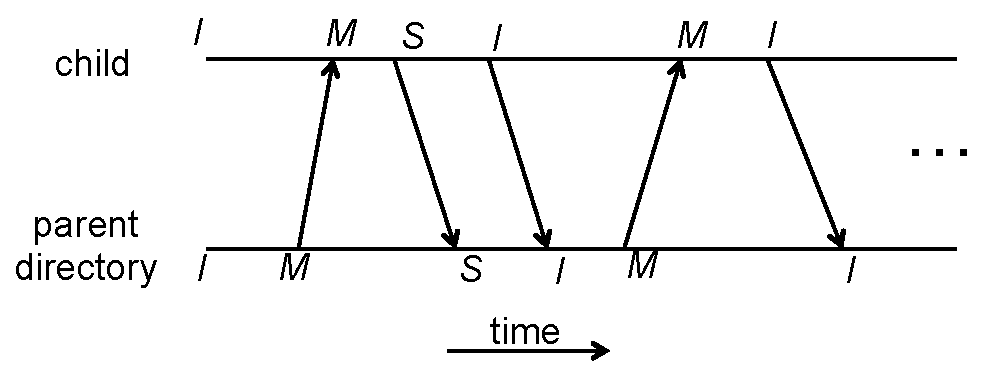
\includegraphics[scale=.45]{resps}
\caption{An example showing a sequence of responses between a child and its parent}
\label{resps}
\end{figure}

Figure~\ref{resps} shows an example of the effect of
Invariants~\ref{stateChange}, \ref{noCross} and \ref{respFIFO}. The
directory entry of the parent or the state of the child changes on sending and
receiving a response, and the new state is shown at the points of sending or
receiving responses.  Both the cache and its parent follow the same sequence of
state and directory entry changes, but the receiver always lags slightly behind
the sender.  The receiver cannot send any response before receiving because of
Invariant~\ref{noCross}, thereby eliminating any scenarios where the lag
complicates reasoning.

Using these three invariants (Invariants~\ref{stateChange}, \ref{noCross} and
\ref{respFIFO}), it is easy to see that Lemma~\ref{conservative} holds.
Intuitively, going back to Figure~\ref{resps}, we can see that at all times,
either there is no response in flight, only responses from the parent are in
flight, or only responses from the child are in flight. A response from child
downgrades the state, and a response from parent upgrades the directory. Since
the other side simply lags behind, Lemma~\ref{conservative} holds.
Since Invariants~\ref{stateChange}, \ref{noCross} and \ref{respFIFO} deal with
just one cache's state for a single address and the corresponding directory
entry, these properties can also potentially be verified using model-checking.
Thus, if some other protocol is verified to obey Invariants~\ref{stateChange},
\ref{noCross} and \ref{respFIFO} using model-checking, then
Lemma~\ref{conservative} is already automatically verified for that
protocol.

Analyzing a parent-child pair will suffice in proving
Lemmas~\ref{localCompatibility1} and \ref{localCompatibility2}.  Proof of
Lemma~\ref{noTransitWrite} is similar to the proof of
Lemma~\ref{nonAncestorCompatible}.

%Figure \ref{something} gives the structure of the proof for Theorem \ref{ccorrect}
%\begin{figure*}
%\begin{prooftree}
%\AxiomC{stateChange}
%\AxiomC{noCross}
%\AxiomC{respFifo}
%\TrinaryInfC{conservative}
%\AxiomC{localCompatibility1}
%\AxiomC{localCompatibility2}
%\TrinaryInfC{nonAncestorCompatible}
%\AxiomC{noTransitWrite}
%\BinaryInfC{latestValue}
%\AxiomC{$\ldots$ (trivial)}
%\BinaryInfC{StoreAtomicity}
%\UnaryInfC{$M_c \sqsubseteq M_m$}
%\end{prooftree}
%\caption{Proving $M_c \sqsubseteq M_m$}
%\label{something}
%\end{figure*}

\section{The Final Result}\label{sec:finalresult}

With our two main results about optimized processors and memories, it
is now straightforward to complete the correctness proof of the
composed optimized system.

First, we need to know that, whenever the simple memory can generate
some trace of messages, it could also generate the same trace with all
speculative messages removed.  We need this property to justify the
introduction of speculation, during our final series of refinements
from the optimized system to SC.

\begin{theorem}
\label{mcorrect}
$M_m \sqsubseteq_{\noSpec^n} M_m$
\end{theorem}
\begin{proof}
By induction on traces, with an identity abstraction function.
\end{proof}

That theorem turns out to be the crucial ingredient to justify placing
a speculative processor in-context with simple memory.

\begin{theorem}
\label{ocorrect1}
$\text{P$^n_\text{so}$} + M_m \sqsubseteq \text{P$^n_\text{ref}$} + M_m$
\end{theorem}
\begin{proof}
Follows from Theorem \ref{liftplus} (one of our preliminary results
about $+$), Corollary \ref{ges}, and Theorem \ref{mcorrect}.
\end{proof}

The last theorem kept the memory the same while refining the
processor.  The next one does the opposite, switching out memory.

\begin{theorem}
\label{ocorrect2}
$\text{P$^n_\text{so}$} + M_c \sqsubseteq \text{P$^n_\text{so}$} + M_m$
\end{theorem}
\begin{proof}
Follows from Theorems \ref{ccorrect} and \ref{liftplus} plus reflexivity of $\sqsubseteq$ (Theorem \ref{transitive}).
\end{proof}

\begin{theorem}
\label{ofull}
$\text{P$^n_\text{so}$} + M_c \sqsubseteq SC$
\end{theorem}
\begin{proof}
We twice apply $\sqsubseteq$ transitivity (Theorem \ref{transitive}) to
connect Theorems \ref{ocorrect2} and \ref{ocorrect1}, and use Definition \ref{sc} of $SC$
\end{proof}

\section{Architectural Implications}\label{sec:implications}

We have demonstrated a high-performance implementation of SC with
a distributed shared-memory system and speculative processors. However, here
are some of the concerns that an architect of a high-performance multi-processor
may have about our design:

\begin{enumerate}
\item Splitting each load into a speculative load and a verification
load increases the number of requests to the L1 cache. While verification loads
are extremely likely to hit in a cache and therefore have low latency,
nevertheless they fundamentally increase cache pressure on L1. Can we
eliminate some of this verification traffic?

\item The correctness of our model with respect to sequential consistency
crucially relies on the fact that a commit operation for only one load or store
can be active per processor at a time. Can we pipeline commit requests, \ie{}
have several of them issued at a time?

\item In some designs, a processor does not receive an explicit acknowledgement
for a store operation. Intuitively the store acknowledgment means that a store
has been placed in a global order of all stores being issued to the memory, and
this condition can potentially be determined even before the data is stored in
any cache. Can this optimization be incorporated in our framework?
\end{enumerate}

A trick architects use to reduce the need for verification loads is to use the
invalidation signal received by L1 (\eg{} in the MIPS R10000 processor~\cite{yeager1996mips}) 
to invalidate speculative loads for that address in the reorder buffer. 
The reason this works is that such a signal is an
indicator of the fact that another processor has changed the value of that
address before the load has been committed. This scheme is simultaneously
incomplete, in that it does not alleviate the need for verification loads in the
context of address speculation; and conservative, in that it invalidates loads
whose values may not have changed in spite of a write into the corresponding
cache line. Incorporating this solution will require a very small change in our
processor interface, \viz{} that of including invalidation signals from L1
caches.

The solutions for the remaining two issues require making some extra
assumptions about the memory interface. These assumptions can be enforced by
having an extra module (Load Store Buffer, LSB) in front of the memory we have
presented. The processor can issue a commit store request to the LSB and
assume that it receives the acknowledgment straightaway, continuing to issue
further commit requests to the LSB. A verification load request in the LSB
still has to receive a response from L1. It will be sent to L1 only after all
previous commit store requests in the LSB have been sent to L1. The formal
proof of why this scheme works is beyond the scope of this paper.

A more aggressive solution to maintaining the strict load-store orderings
defined by SC is to change the memory model itself. Indeed, many processors use
a more relaxed memory model; for instance, Intel x86 and Sparc use
TSO~\cite{intel64and,weaver1994sparc}, ARM and PowerPC both use their own
relaxed memory models~\cite{grisenthwaite2009arm,power2009version}.
Two things need to be noted about all relaxed memory models. First, every SC
behavior is
always a legal behavior in a relaxed model, making our speculating processor
correct in such a setting. Second, the ISA must be augmented with explicit
memory fence instructions that prevent reorderings of memory instructions
across fences, if the application demands preserving the order. Adding explicit memory fences is generally slower than implicitly
having the restrictions within the memory model, but the belief is that
explicit fences are only needed sparingly in practice and on the whole will
give better performance than the equivalent SC system.
%\murali{Starting from "two things", the rest seems out of place}

In order to use our methodology for systems with relaxed memory models, we
would have to provide an LTS description for each model. One can potentially
adjust our processor model accordingly (for
instance, more aggressive issue of even verification loads) and add the LSB described
earlier. The details are not obvious, however. Alglave
\etal{}~\cite{alglave2012formal,alglave2014herding} provide a framework for 
axiomatic specification of memory models.  Axioms regarding relaxed memory
models have also been proposed through analysis of empirically observed behavior
of certain ``litmus tests''~\cite{mador2012axiomatic,sarkar2012synchronising}.
There has also been work in providing operational semantics that describe the
observed behavior of real hardware~\cite{sarkar2011understanding}, and proving
the equivalence between the axiomatic specification of TSO and operational
semantics of a simple in-order processor with a store buffer and instantaneous
global memory~\cite{x86tsocacm10}. However, others have suggested
simplifying memory models, in other words to implement SC in real
hardware~\cite{hill1998multiprocessors}.

\section{Related Work}
\label{relatedWork}

Formal verification has been used to verify multiprocessor
systems, especially with model checking
\cite{burch1994automatic,mcmillan1998verification}.

More recently, Intel's execution cluster (\ie{} the ALU and its
interface) has been formally verified using model checking
\cite{kaivola2009replacing}.

Theorem provers have also been used to verify microprocessors, \eg{} HOL has been
used to verify an academic microprocessor AVI-1 \cite{windley1995formal}.
Term-rewriting based techniques have been used to specify microprocessors, with
the goal of making them more amenable to verification \cite{shen1999using}.

%\murali{Next paragraph is all I know about this stuff, should probably be
%removed}
%\adam{What are you referring to with ``it'' in your comment?  I don't understand what this paragraph refers to.}
%It has been verified using model checking \cite{qadeer2003verifying},
%with a fixed number of processors and memory locations.  Model-checking has also
%been used to verify communication fabrics \cite{chatterjee2012automatic}.


Theorem provers have also been used in verifying cache coherence protocols.
The correctness of the FLASH cache coherence protocol~\cite{flash} for a
single-level hierarchy was proven with PVS~\cite{park} using a mapping, called
``aggregation of transactions,'' from multiple localized transactions to a
single global transaction, and finally using model checking to prove the correctness of
the global transactions model. However, they do not provide a methodology to
prove the aggregation of transactions for other protocols, which is where, we
believe, the difficulty lies; in contrast, our modular proof relies on generic
invariants, making it more adaptable to different protocols.

Cachet~\cite{StoyShenArvind:Proofs}, another single-level cache coherence
protocol, was proven to be implementable in the CRF memory
model~\cite{Shen:CRF}. Shen \etal{} provided a paper-and-pencil proof showing
Cachet does not violate the CRF memory model, while Stoy \etal{} implemented
portions of the paper-and-pencil proof using PVS. However, neither proof
establishes that the protocol is store atomic. Rather, they show that Cachet
obeys the CRF memory model, which is not restricted to store-atomic behavior.


%There has been a lot of work in providing frameworks for axiomatic
%specifications of memory models \cite{alglave2012formal,alglave2014herding}
%and in providing axiomatic memory model specifications for real systems
%through analyis of empirically observed behavior of certain ``litmus tests''
%\cite{mador2012axiomatic,sarkar2012synchronising}. There has also been some
%work in providing operational semantics that describes the observed behavior of
%real hardware \cite{sarkar2011understanding}. Finally, there has been work
%formally relating the axiomatic specification of TSO to operational semantics
%of real x86 and Sparc machines \cite{x86tsocacm10}.
%
%The plethora of work in the area of memory models indeed suggests that this is
%a complex problem, exacerbated by the hardware architect's desire to increase
%hardware performance at the cost of complicating the memory models further. There
%are two aspects where our work can help in tackling this complex problem: (1) we
%are proposing a modular approach for verifying systems in which the components,
%namely the processors and the memory, can be verified against the memory model
%contract independent of each other, and (2) we are also proposing a design
%in which a system obeying sequential consistency is made into a high
%performance machine through the use of speculative loads followed by
%verification. The only downside is waiting for store acknowledgements, but this
%wait does not preclude the machine from performing further computations for
%future instructions without actually committing them. We are hoping to develop
%both these ideas -- of extending our proof approach for more complex memory
%models and designing real hardware which is sequentially consistent but has
%high performance.
%
%
%BELOW IS UNEDITTED FROM OLD PAPER


%These are lifted as is from that guy. Need to figure out how to restate them, and make it more concise.
%
%For verification of high level specifications, modern industrial practice
%consists of modeling small instances of the protocols, e.g., three CPUs
%handling two addresses and one bit of data, in terms of interleaving atomic
%steps, in guard/action languages such as Murphi [50] or TLA+ [84], and
%exploring the reachable states through explicit state enumeration.
%Symbolic methods, e.g., BDD [31] or SAT [129, 142], are yet to succeed for the
%verification of cache coherence protocols.
%Monolithic formal verification methods – methods that treat the protocol as a whole – have
%been used fairly routinely for verifying cache coherence protocols from the early 1990s
%[10 (2 nodes, murphi)]. However, these monolithic techniques will not be able to handle the very
%large state space of hierarchical protocols. Compositional verification techniques are essential. 
%
%For coherence protocols which only consider one level (or nonhierarchical protocols),
%various techniques have been proposed for the verification. These techniques basically
%include explicit state enumeration [133] and symbolic model checking [102]
%Opti-
%mizations on these techniques include partial order reduction [24], symmetry reduction
%[25, 72], compositional reasoning [96], predicate abstraction [22, 49, 82], etc. There is
%also a large body of work on parameterized verification [42, 53, 54, 100, 117]. However,
%none of them have shown the capability to verify hierarchical coherence protocols with
%realistic complexity.
%
%McMillan et al. [97, 102] modeled a 2-level MSI coherence protocol based on the
%Gigamax distributed multiprocessor [102]. In the protocol, bus snooping is used in both
%levels. SMV [97] was used to verify this protocol with two clusters each having six
%processors, for both safety and liveness properties. In terms of the complexity, many
%realistic details are abstracted away from the protocol so that the protocol does not have
%the typical complexity that a hierarchical coherence protocol has.
%
%=======
%Theorem provers have also been used in verifying cache coherence protocols,
%\eg{} FLASH~\cite{park} and Cachet~\cite{Shen:CRF, StoyShenArvind:Proofs} have
%been proved using the PVS theorem prover. Both works prove correctness of a
%single-level hierarchy while our work proves it for a multi-level hierarchy.
%The work by Park \etal{} on FLASH proves a mapping, called ``aggregation of
%transactions'', from multiple localized transactions to a single global
%transaction with PVS, and uses model-checking to prove the correctness of the
%global transactions model. However, they do not provide a methodology to prove
%the aggregation of transactions for other protocols, which we believe to be very
%difficult; in contrast, our modular proof relies on generic invariants making it
%more naturally adaptable to different protocols.
%>>>>>>> 96e9880a190d9acb6201b10e2b105d18c72f56aa

\section{Conclusions and Future Work}\label{sec:conclusion}

In this paper we developed a modular proof structure for distributed
shared-memory hardware systems, corresponding naturally to the modularization seen in
hardware implementations. Our approach allows verification of the
system to be carried out throughout the implementation process without
disrupting the architect's design process.

While we provide a clean interface for an SC system, we are working on
encompassing relaxed memory models commonly used in a modern processors.

Another direction that bears investigation is extending our results to
cover finer-grained architectural details.
However, the behaviors of microarchitectural structures,
\ie{} register renaming structures \etc{}, vary significantly across
implementations and can be quite complex. It is not clear if a
practical modularization can be found that strikes a balance between flexibility and
simplicity.

Finally, to make full use of our results for implementations, hardware
descriptions must be translated to and from our labeled transition system
representation. As we implied in the discussion of our cache-coherence system,
Bluespec SystemVerilog's rule-based representation is very close to LTSes and
in some cases can be transliterated directly.  There has been work to generate
circuits from Bluespec-like descriptions in Coq \cite{Braibant2013Fesi} and we
are pursuing further automatization.

%%\subsection*{Acknowledgments}
{\footnotesize\noindent\textbf{Acknowledgments:} The parts of this work done
at MIT was supported by Quanta Research agreement dated 4/1/05 and
Angstrom Project under Grant No. HR0011-10-9-0009. The research at SRI
was supported by Defense Advanced Research Projects Agency (DARPA) and
Air Force Research Laboratory (AFRL), under contract FA8750-11-C-0249
and National Science Foundation under Grant No. CCF-1217498. The
views, opinions, and/or findings contained in this report are those of
the authors and should not be interpreted as representing the official
views or policies, either expressed or implied, of the Quanta
Research, the Defense Advanced Research Projects Agency, the United
States Air Force or the Department of Defense. We would like to thank
Richard Uhler for helping focus this paper in early drafts.% }
%
%{ We would like to thank Richard Uhler for helping focus this paper in
%  early drafts.  This work was supported by the Defense Advanced
%  Research Projects Agency (DARPA) and the United States Air Force,
%  under Contract No. FA8750-11-C-0249. Any opinions, findings and
%  conclusions or recommendations expressed in this material are those
%  of the authors and do not necessarily reflect the views of DARPA or
%  the United States Air Force.  }


\input{Appendix}


%=========================================================================
%  Bibliography
%=========================================================================

% When using Bibtex, the following form may be used.

\bibliographystyle{abbrvnat}
\bibliography{refs}



%=========================================================================
%  Appendix
%=========================================================================

%\pagebreak \small

\begin{appendix}
\input{Appendix}
\end{appendix}

\end{document}
